%%%%%%%%%%%%%%%%%%%%%%%%%%%%%%%%%%%%%%%%%%%%%%%%%%%%%%%%%%%%%%%%%%%%%%
%%% methods.tex
%%% 数値計算法
%%%%%%%%%%%%%%%%%%%%%%%%%%%%%%%%%%%%%%%%%%%%%%%%%%%%%%%%%%%%%%%%%%%%%%
%%%
%%%%%%%%%%%%%%%%%%%%%%%%%%%%%%%%%%%%%%%%%%%%%%%%%%%%%%%%%%%%%%%%%%%%%%
\chapter{数値計算法}
\label{chap:methods}
%%%%%%%%%%%%%%%%%%%%%%%%%%%%%%%%%%%%%%%%%%%%%%%%%%%%%%%%%%%%%%%%%%%%%%
%%%  main.tex から\include : YaTeX 用コマンド
%#!platex main.tex
%%%%%%%%%%%%%%%%%%%%%%%%%%%%%%%%%%%%%%%%%%%%%%%%%%%%%%%%%%%%%%%%%%%%%%
本章では,軌道計算・Navier–Stokes解析・DSMC法における数値計算法について述べる.


\section{軌道計算の数値計算法}
\subsection{支配方程式}
軌道上を周回する人工衛星から進行方向後ろ向きに放出された流星源は,放出された地点を遠地点とした楕円軌道に投入される. 放出された流星源の運動方程式は,流星源の位置$\bm{r}$, 速度$\bm{v}$, 質量$m$を用いて以下のように記述される.
\begin{equation}
    \label{eq:equation-of-motion}
    m\dfrac{\mathrm{d}^2\bm{r}}{\mathrm{d}t^2} = -\nabla U(\bm{r}) - \dfrac{1}{2}C_\mathrm{d} S \rho \bm{v}^2\dfrac{\bm{v}}{|\bm{v}|}.
\end{equation}
ここで, $C_\mathrm{d}$は抗力係数, $S$は前面投影面積, $\rho$は大気密度であり, $U(\bm{r})$は地球の重力ポテンシャルである.

流星源は大気圏突入時に空力加熱を受け,アブレーションを起こす. アブレーションによる質量減少は以下のように表される.
\begin{equation}
    \label{eq:mass-by-ablation}
    L^*\dfrac{\mathrm{d}m}{\mathrm{d}t} = -\dfrac12C_\mathrm{h}S\rho v^3.
\end{equation}
 ただし,$C_\mathrm{h}$は単位時間当たりに流星源に供給されるエネルギーのうち,アブレーションに必要となるエネルギーの割合で,熱伝達係数と呼ばれる.$L^*$は流星源が融解,気化及び破砕を含むアブレーションを起こすために単位質量当りに必要になるエネルギーである.
 
さらに,質量の減少に伴って体積および投影面積も変化する.前面投影面積と質量は形状変化係数$\nu$を用いて,次式に従う.
\begin{equation}
    \label{eq:area-mass}
    \dfrac{S}{S_e} = \left(\dfrac{m}{m_e}\right)^\nu.
\end{equation}
ここで,$S_e$と$m_e$はそれぞれ人工衛星から放出された直後の前面投影面積と質量である.

本研究では,アブレーションによる質量減少過程において形状は変化せず,球形を保ったままであると仮定した.加えて流星源は質量密度が一様であると仮定すれば形状変化係数は以下のようになる.
\begin{equation}
    \label{eq:shape-coeff}
    \nu = \dfrac23.
\end{equation}
これは,球の質量は半径の3乗に比例し,前面投影面積は半径の2乗に比例するためである.

流星の発光強度は運動エネルギー$E$を用いて以下のように表される~\cite{popova2004meteoroid}.
\begin{equation}
	\label{eq:brightness}
	I = -\tau\dfrac{\mathrm{d}E}{\mathrm{d}t} = -\tau\left(\dfrac{v^2}{2}\dfrac{\mathrm{d}m}{\mathrm{d}t} + mv\dfrac{\mathrm{d}v}{\mathrm{d}t}\right).
\end{equation}
ここで$\tau$は発光効率と呼ばれるパラメータで,運動エネルギーがどれだけ発光に寄与するかを示す.
発光効率の正確な見積もりは未だ研究途上であるため,本シミュレータでは便宜的に$\tau = 0.01$とした.
また,流星の発光効率に関する理論的な知見は研究段階であり~\cite{subasinghe2017luminous,subasinghe2018luminous,revelle2001bolide},発光効率の見積もりには,空力計算とアブレーション計算の連成解析が必要になる.

\subsection{熱流束モデル}
流星源は極超音速で大気圏に突入するため,強い衝撃波が前方に形成され,空力加熱を受ける.
この空力加熱は,流動によって行われる対流加熱と,高温により励起された原子が脱励起する際に放出する電磁波によって加熱される輻射加熱に分けられる.
流星源は天然のものよりも低速で運動するため,本研究では対流加熱のみを考慮した.
対流加熱による加熱率のモデルには,次式に示すDetra–Kemp–Riddle~\cite{kemp1957heat} の推算式(DKRモデル, 冷壁条件)を用いた.

\begin{equation}
    \label{eq:dkr-model}
	q= \dfrac{110.35}{\sqrt{r}} \left(\dfrac{v}{v_\mathrm{ref}}\right)^{-3.15}\left(\dfrac{\rho}{\rho_\mathrm{ref}}\right)^{0.5}.
\end{equation}
ここで,$r$は球半径で,$v_\mathrm{ref} = 7,925$~m/s,$\rho_\mathrm{ref} = 1.225$~kg/m$^3$である.この式は軌道から決まる速度と大気密度を用いて対流加熱を見積もることが可能なため,再突入設計においてよく用いられる~\cite{nagoya-twins}.

\subsection{抗力係数モデル}
次に抗力係数について述べる.宇宙空間で周回する人工衛星に限っては,抗力係数は経験的に2前後であることが分かっているが,再突入物体に対しては抗力係数は定数ではなく軌道上で大きく変動することが分かっている.特に自由分子流から連続流へと遷移する領域は空気力学的にも熱力学的にもさまざまな変化が起こる領域であり,そこでの抗力係数の挙動の詳細は明らかでない.

Hendersonによると,Mach数が1.75以上の超音速領域における抗力係数$C_\mathrm{d}$は以下に示すようにMach数$M$, Reynolds数$Re$の関数として求められる~\cite{henderson1976drag}.
\begin{align}
    \label{eq:drag-coeff}
    C_\mathrm{d} &= \dfrac{0.9 + \dfrac{0.34}{M^2} + 1.86\sqrt{\dfrac{M}{Re}}\left[ 2 + \dfrac{2}{Sa^2} + \dfrac{1.058}{Sa}\sqrt{\dfrac{T_\mathrm{w}}{T}} - \dfrac{2}{Sa^4} \right]}{1 + 1.86\sqrt{\dfrac{M}{Re}}}, \\
    Sa &= M\sqrt{\dfrac{\gamma}{2}}.
\end{align}
ここで$\gamma$は空気の比熱比であり,$T_\mathrm{w}$は流星源の表面温度,$T$は大気温度である.

\subsection{熱伝達係数モデル}
熱伝達係数は流星源の質量減少に関与するパラメータの一つであるが,その詳細な知見は未だ得られていない.
Pageら~\cite{page1969radiative}やBaldwinら~\cite{baldwin1971ablation}が導出した0.1という値はひとつの指標となっており,Johnstonらが数値流体計算により流星再突入を模擬した際も,熱伝達係数の比較対象として0.1を選んでいる~\cite{johnston2018radiative}.

Prevereaudによると,熱伝達係数$C_\mathrm{h}$は次式のように,Mach数$M$の関数として表される~\cite{prevereaud2016phd}.
\begin{align}
    \label{eq:heat-coeff}
    C_\mathrm{h} &= \dfrac{2q}{\rho v^3}\dfrac{I_1}{I_2},\\
    I_1 &= \int_0^{\frac{\pi}{2}}\left\{\left( \sin^2\theta + \dfrac{\cos^2\theta}{1+\zeta M^2} \right)\left(\dfrac{\pi}{2} - \theta\right)\cos\theta\sin\theta\right\}\mathrm{d}\theta,\\
    I_2 &= \int_0^{\frac{\pi}{2}}\left\{\left( \sin^2\theta + \dfrac{\cos^2\theta}{1+\zeta M^2} \right)\left(\dfrac{\pi}{2} - \theta\right)\cos^2\theta\right\}\mathrm{d}\theta.
\end{align}
ここで,$q$は流星源が受ける熱流束であり,先に示したDKRモデルでの見積もりを使用する.

\subsection{大気モデル}
本軌道計算シミュレータにおいて,大気密度及び大気温度はそれぞれ抗力・熱伝達係数の見積もりに必要となる.本研究では大気モデルとして米国海軍研究所 (U.S. Naval Research Laboratory: NRL) が公開している経験モデル NRLMSISE–00 を使用する.本モデルにおける入力パラメータとしては時刻・座標に加えて,太陽活動指数と磁気指数が挙げられる.

太陽は約11年周期で活発期と静穏期を繰り返している.太陽活動の指標として黒点の数が広く用いられている.
黒点数も約11年周期で変動しており,黒点数が多い時期には太陽活動は活発となり太陽フレアも起きやすくなる.
また,古くからF10.7と呼ばれる値も太陽活動の指標として利用されている.
このF10.7は太陽から定常的に放射されている波長10.7~cm (2.8~GHz)の電磁場強度でSolar Flux Unit ($10^{22}~\mathrm{W/m^2Hz}$)という単位で表され,この値は黒点数と非常に良い相関があることが知られている.

また,地磁気の強度は常に変化しており,太陽活動と同じく11年周期で変動を繰り返しているほか,27日周期,1日周期といった短い期間でも変動している.
さらに,数日間に渡って非常に地磁気が乱れる地磁気擾乱が起こることもあり,こうした複雑な地磁気活動度を準対数的に表現しようとするKp指数がある.
Kp指数は1949年頃Bartlesによって考案された指数で,現在はドイツの Geo Forschungs Zentrum~\cite{GeoForschungsZentrum} によって算出されている.
この指数はサブオーロラ帯に位置する13ヶ所の観測所で観測された地磁気データから3時間ごとに算出され,各観測所における地磁気擾乱の振幅を対数的に表現した後,それらの平均値を28段階に表したものである.
地磁気擾乱の程度を表す指標として広く用いられているほか,地磁気静穏日・擾乱日の決定にも使用される.Kp指数は地磁気擾乱の振幅に対して対数的に応答するが,これを線形で表したのがap指数である.
1日分の8個のap指数の平均値がAp指数と呼ばれる日単位の指数である~\cite{GeoForschungsZentrum}.

海洋と大気に関する調査および研究を行っているアメリカ海洋大気庁 (National Oceanic and Atmospheric Administration: NOAA) の宇宙天気予報センター (Space Weather Prediction Center: SWPC~\cite{SWPC-NOAA}) はF10.7,Ap指数の変動について2000年から2018年までの記録に2019年の予測を加えた10年分のデータを公開しており,
太陽活動及び地磁気活動のの約1周期分を確認できる.
また,太陽活動が極大期を迎えた約2年後に地磁気の擾乱が起きることが読み取れ,これは藤田~\cite{fujita2007taiyou}によって指摘されている.

太陽活動が活発であるほど,また地磁気擾乱時ほど,大気密度と大気温度は高くなる.反対に,太陽活動や地磁気が静穏であるほど,大気密度と大気温度は低くなる.
木村\cite{kimura2018master}は,太陽活動極大期および地磁気擾乱時の条件としてF10.7 $=$ 240, Ap指数を40,太陽活動極小期および地磁気静穏時の条件としてF10.7 $=$ 60, Ap指数を1と仮定して比較を行った.
結果として高高度において特に大気温度が顕著な違いを示した一方で,流星源速度や質量減少率,流星源が受ける加熱率にはほとんど影響を及ぼさなかった.

従って本研究では,条件として太陽活動極大期および地磁気擾乱時の条件であるF10.7 $=$ 240, Ap指数を40とする.

\subsection{離散化手法}
支配方程式である微分方程式の解析手法としては4段4次の陽的Runge–Kutta法を用いた.解きたい微分方程式が$\frac{\mathrm{d}y}{\mathrm{d}t} = f(t,y)$である時,Runge–Kutta法は次式で表される.
\begin{align}
    \label{eq:runge-kutta}
    y_{n+1} &= y_n + h\sum^s_{i=1}b_ik_i, \\
    k_i &= f\left(t_n + hc_i, y_n + h\sum_{j=1}^s a_{ij} k_j\right), \quad i = 1,\ldots,s.
\end{align}
ここで$n$は時間ステップ,$h$は時間刻み幅,$s$は段数である.
また,$a_{ij}$は係数,$b_i$は重み,$c_i$は節点であり,本研究で用いた4段4次の陽的Runge–Kutta法においてはそれぞれ次のブッチャー配列で与えられる.
\begin{equation}
    \begin{array}{c|c} \bm c & A \\ \hline & \bm b^\top \end{array} =
    \begin{array}{c|ccccc} c_1 & a_{11} & a_{12} & \cdots & a_{1s} \\ c_2 & a_{21} & a_{22} & \cdots & a_{2s} \\ \vdots & \vdots & \vdots & \ddots & \vdots \\ c_s & a_{s1} & a_{s2} & \cdots & a_{ss} \\ \hline & b_1 & b_2 & \cdots & b_s \end{array} =
    \begin{array}{c|cccc} 0 & 0 \\ 1/2 & 1/2 & 0 \\ 1/2 & 0 & 1/2 & 0 \\ 1 & 0 & 0 & 1 & 0 \\ \hline & 1/6 & 1/3 & 1/3 & 1/6 \end{array}
\end{equation}
ただし,上三角行列は全て0になるので省略した.
また,Runge–Kutta法においての時間刻み幅は木村~\cite{kimura2018master}により\SI{1e-2}{s}で収束することが確かめられており,本研究においても\SI{1e-2}{s}を用いる.


\newpage
\section{Navier–Stokes 解析の数値計算法}
\subsection{支配方程式}
流体を連続体とみなした際の支配方程式は,以下に示す2次元軸対称圧縮性Navier–Stokes方程式である.
\begin{equation}
   \dfrac{\partial {\bm Q}}{\partial t}
  +\dfrac{\partial ({\bm F}-{\bm F}_\mathrm{vis})}{\partial x}
  +\dfrac{\partial ({\bm G}-{\bm G}_\mathrm{vis})}{\partial y}
  +\dfrac{1}{y}({\bm H}-{\bm H}_\mathrm{vis})
  ={\bm W}.
  \label{tab:goveq}
\end{equation}
ここで,
${\bm Q}$は保存量ベクトル,
${\bm F}$, ${\bm G}$は対流流束ベクトル,
${\bm F}_\mathrm{vis}$, ${\bm G}_\mathrm{vis}$は粘性流束ベクトル,
${\bm H}$, ${\bm H}_\mathrm{vis}$はそれぞれ三次元圧縮性 Navier–Stokes 方程式を軸対称表記した際に対流流束と粘性流束から現れる項,
${\bm W}$は生成項であり,
以下のように与えられる.
\begin{equation}
  {\bm Q}=
  \begin{pmatrix}
  \rho\\
  \rho u\\
  \rho v\\
  E\\
  \rho_s\\
  E_{v}+E_{el}
  \end{pmatrix},
\end{equation}
%
\begin{equation}
  {\bm F}=
  \begin{pmatrix}
  \rho u\\
  \rho u^2+p\\
  \rho u v\\
  (E+p) u\\
  \rho_s u\\
  \left(E_{v}+E_{el}\right)u
  \end{pmatrix},
  {\bm G}=
  \begin{pmatrix}
  \rho v\\
  \rho u v\\
  \rho v^2+p\\
  (E+p) v\\
  \rho_s v\\
  (E_{v}+E_{el})v
  \end{pmatrix},
  {\bm H}=
  \begin{pmatrix}
  \rho v\\
  \rho u v\\
  \rho v^2\\
  (E+p) v\\
  \rho_s v\\
  (E_{v}+E_{el})v  
  \end{pmatrix},
\end{equation}
%
\begin{eqnarray}
  {\bm F}_\mathrm{vis}&=&
  \begin{pmatrix}
  0\\
  \tau_{xx}\\
  \tau_{xy}\\
  u\tau_{xx}+v\tau_{xy}-q_{tx}-q_{vx}-\sum_{s}\rho_{s}u_{s}h_{s}\\
  -\rho_{s}u_{s}\\
  -q_{vx}-\sum_{s}\rho_{s}u_{s}(e_{vs}+e_{els})
  \end{pmatrix}\nonumber,\\
  {\bf G}_v&=&
  \begin{pmatrix}
  0\\
  \tau_{yx}\\
  \tau_{yy}\\
  u\tau_{yx}+v\tau_{yy}-q_{ty}-q_{vy}-\sum_{s}\rho_{s}v_{s}h_{s}\\
  -\rho_{s}v_{s}\\
  -q_{vy}-\sum_{s}\rho_{s}v_{s}(e_{vs}+e_{els})
  \end{pmatrix},\\
  {\bm H}_\mathrm{vis}&=&
  \begin{pmatrix}
  -\rho_{s}v_{s}\\
  \tau_{xy}\\
  \tau_{yy}-\tau_{\theta \theta}\\
  u\tau_{xy}+v\tau_{yy}-q_{ty}-q_{vy}- \sum_{s} \rho_{s}v_{s}h_{s}\\
  -\rho_{s}v_{s}\\
  -q_{vy}-\sum_{s}\rho_{s}v_{s}(e_{vs}+e_{els})
  \end{pmatrix}\nonumber,
\end{eqnarray}
%
\begin{equation}
  {\bm W}=
  \begin{pmatrix}
  0\\
  0\\
  0\\
  0\\
  {\dot W}_{s}\\
  {\dot W}_{v}
  \end{pmatrix}.
  \label{tab:termgen}
\end{equation}
%
ここで,
$\rho~\mathrm{[kg/m^3]}$は密度,
$u,\ v~\mathrm{[m/s]}$はそれぞれ$x,\ y$方向の速度成分,
$E~\mathrm{[J/m^3]}$は単位体積あたりの全エネルギー, 
$\rho_s~\mathrm{[kg/m^3]}$は化学種$s$の密度,
$E_v~\mathrm{[J/m^3]}$は単位体積あたりの振動エネルギー, 
$E_{el}~\mathrm{[J/m^3]}$は単位体積あたりの電子エネルギーを表し, 
$p~\mathrm{[Pa]}$は圧力,
$\tau~\mathrm{[N/m^2]}$は粘性応力,
$u_s,\ v_s~\mathrm{[m/s]}$はそれぞれ化学種$s$の拡散速度の$x,\ y$方向成分,
$q_t$は並進$\cdot$回転熱流束,
$q_v$は振動$\cdot$電子励起熱流束,
$h_s$は化学種$s$の単位質量あたりのエンタルピー,
$e_{vs}$は化学種$s$の振動エネルギー,
$e_{els}$は化学種$s$の電子励起エネルギー,
$W_s$は化学種$s$の生成量,
$W_v$は振動$\cdot$電子励起エネルギーの生成量を表す.
%
粘性応力$\tau$は,
Stokes の定理を用いて以下のように与えられる.
\begin{eqnarray}
  &&\tau_{xx}=\dfrac{2}{3}\mu \left( 2\dfrac{\partial u}{\partial x}-\dfrac{\partial v}{\partial y}-\dfrac{v}{y} \right),\\
  &&\tau_{xy}=\tau_{yx}=\mu \left( 2\dfrac{\partial u}{\partial y}+\dfrac{\partial v}{\partial x} \right),\\
  &&\tau_{yy}=\dfrac{2}{3}\mu \left( 2\dfrac{\partial v}{\partial y}-\dfrac{\partial u}{\partial x}-2\dfrac{v}{y} \right),\\
  &&\tau_{\theta \theta}=\dfrac{2}{3}\mu \left( \dfrac{\partial v}{\partial y}-\dfrac{\partial u}{\partial x}+2\dfrac{v}{y} \right).
\end{eqnarray}
ここで,
$\mu$は粘性係数を表す.
%
並進・回転熱流束$q_t$,
振動・電子励起熱流束$q_v$は Fourier の法則より以下のように与えられる.
\begin{align}
q_{tx}&=-\kappa_{tx}\dfrac{\partial{T}}{\partial{x}},\\
q_{ty}&=-\kappa_{ty}\dfrac{\partial{T}}{\partial{y}},\\
q_{vx}&=-\kappa_{vx}\dfrac{\partial{T_v}}{\partial{x}},\\
q_{vy}&=-\kappa_{vy}\dfrac{\partial{T_v}}{\partial{y}}.
\end{align}
ここで,
$T$は並進・回転温度,
$T_v$は振動・電子励起温度,
$\kappa_t$は並進・回転温度に対する熱伝導係数,
$\kappa_v$は振動・電子励起温度に対する熱伝導係数を表す.
%
化学種の拡散速度$u_s,\ v_s$は Fick の法則より以下のように与えられる.
\begin{align}
\rho_{s}u_{s}=-\rho D_s\dfrac{\partial{c_s}}{\partial{x}},\\ 
\rho_{s}v_{s}=-\rho D_s\dfrac{\partial{c_s}}{\partial{y}}.
\end{align}
ここで,
$D_s$は化学種$s$の拡散係数を表す.

本計算では,
\ce{O}, \ce{N}, \ce{NO}, \ce{O2}, \ce{N2}の 5 化学種の内,
\ce{O}, \ce{N}, \ce{NO} の 3 化学種についての質量保存の式を解く.
\ce{O2}, \ce{N2}の密度は,
以下の元素組成一定の仮定を用いて得られる.
\begin{align}
\rho_{\ce{O2}} &= M_{\ce{O2}} (\alpha_1 \rho + \alpha_2 \rho_{\ce{O}} + \alpha_3 \rho_{\ce{NO}} ), \\
\rho_{\ce{N2}} &= M_{\ce{N2}} (\alpha_4 \rho + \alpha_5 \rho_{\ce{N}} + \alpha_6 \rho_{\ce{NO}} ).
\end{align}
ここで,
$M_{s}$は化学種$s$の分子量を表し,
パラメーター$\alpha{_i}$は以下のように与えられる.
\begin{align}
\alpha_{1} &=\dfrac{1}{M_{\ce{O2}}+\dfrac{M_{\ce{N2}}}{fr}},\\
\alpha_{2} &=-\alpha_1 \left( 1+\dfrac{1}{2} \dfrac{M_{\ce{N2}}}{M_{\ce{O}}} \right),\\
\alpha_{3} &=-\alpha_1 \left( 1+\dfrac{1}{2fr} \left( \dfrac{1}{fr} -1 \right) \dfrac{M_{\ce{N2}}}{M_{\ce{NO}}} \right),\\
\alpha_{4} &=\dfrac{1}{M_{\ce{N2}}+M_{\ce{O2}}fr},\\
\alpha_{5} &=-\alpha_4 \left( 1+\dfrac{fr}{2} \dfrac{M_{\ce{O2}}}{M_{\ce{N}}} \right),\\
\alpha_{6} &=-\alpha_4 \left( 1-\dfrac{1-fr}{2} \frac{M_{\ce{O2}}}{M_{\ce{NO}}} \right),\\
fr &=\frac{N_{\ce{O}}+2N_{\ce{O2}}+N_{\ce{NO}}} {N_{\ce{N2}}+2N_{\ce{N2}}+N_{\ce{NO}}}.
\end{align}
ここで,
$N_{s}$は化学種$s$のモル濃度であり,
以下のように与えられる.
\begin{equation}
N_s=\dfrac{\rho_s}{M_s}.
\end{equation}

\subsection{輸送係数モデル}
空気を構成する化学種の粘性係数は,
Blottner のモデル\cite{blottner1971chemically}により次のように与えられる.
\begin{equation}
\mu_s=0.1\exp\left[\left(A_s\ln T+B_s\right)\ln T+C_s\right].
\end{equation}
ここで,
定数$A_s$, $B_s$, $C_s$は表~\ref{tab:blocoef}に示す.
それぞれの化学種における並進・回転温度と振動・電子励起温度の熱伝導係数$\kappa_{ts}$, $\kappa_{vs}$は Euken~\cite{kruger1965introduction}の関係式より以下のように求める.
\begin{align}
\kappa_{ts} &=\mu_s \left( \dfrac{5}{2} c_{v{\rm tr}s}+c_{v{\rm rot}s} \right), \\
\kappa_{vs} &=\mu_s c_{v{\rm vib}s}.
\end{align}
ここで,
化学種$s$の並進定積比熱$c_{v{\rm tr}s}$,
回転定積比熱$c_{v{\rm rot}s}$,
振動定積比熱$c_{v{\rm vib}s}$は以下のように与えられる.
\begin{align}
c_{v{\rm tr}s}  &=\dfrac{R}{M_s},\\
c_{v{\rm rot}s} &=\left\{ 
                   \begin{array}{ll}
                      \dfrac{R}{M_s} & {\rm for~\ NO,\ O_2,\ N_2}         \\
                      0 & {\rm for~\ O,\ N}       
                   \end{array} \right.,\\
c_{v{\rm vib}s} &=\left\{ \begin{array}{ll}
                      \dfrac{R}{M_s} & {\rm for~\ NO,\ O_2,\ N_2}         \\
                      0 & {\rm for~\ O,\ N}       
              \end{array} \right. .
\end{align}
ここで,
$R$は一般気体定数($=8.31447$)である.
多成分気体の粘性係数$\mu$および各熱伝導係数$\kappa_{ts}$, $\kappa_{vs}$は Wilke の近似混合則~\cite{wilke1950viscosity}より以下のように求める.
\begin{align}
\mu &=\sum_{s}\dfrac{X_{s}\mu_{s}}{\phi_{s}},\\
\kappa_{ts} &=\sum_{s}\dfrac{X_{s}\kappa_{ts}}{\phi_{s}},\\
\kappa_{vs} &=\sum_{s}\dfrac{X_{s}\kappa_{vs}}{\phi_{s}}.
\end{align}
ここで,
$X_s$はモル分率,
$\phi_s$は補助関数であり,
以下のように定義される.
\begin{align}
X_s &=\dfrac{\dfrac{\rho_s}{M_s}}{\sum_{r}\dfrac{\rho_r}{M_r}} ,\\
\phi_s &=\sum_{r}X_r \left[ 1+\sqrt{\dfrac{\mu_s}{\mu_r}} \left( \dfrac{M_r}{M_s} \right )^{\frac{1}{4}} \right]^2 \left[ \sqrt{8 \left( 1+ \dfrac{M_s}{M_r}\right)} \right]^{-1}.
\end{align}
また,
化学種$s$の拡散係数$D_s$はシュミット数一定($S_c =0.5$)を仮定し,
次式のように与えられる.
\begin{equation}
D_s=\dfrac{\mu}{S_{c}\rho}.
\end{equation}

\begin{table}[H]
 \begin{center}
  \caption{Blottner の粘性係数モデル \cite{blottner1971chemically}}
  \begin{tabular}{c c c c} \hline \hline
    化学種 & $A_s$ & $B_s$ & $C_s$ \\ \hline 
         \ce{O} & 0.0203144 & 0.4294404 & $-$11.6031403 \\
         \ce{N} & 0.0115572 & 0.6031079 & $-$12.4327495 \\
         \ce{NO}& 0.0436378 &$-$0.0335511 &  $-$9.5676430 \\
         \ce{O2}& 0.0449290 &$-$0.0826158 &  $-$9.2019475 \\
         \ce{N2}& 0.0268142 & 0.3177838 & $-$11.3155513 \\ 
         \hline \hline
  \end{tabular}
  \label{tab:blocoef}
 \end{center}
\end{table} 

\subsection{熱化学モデル}
極超音速流れ場中の
物体前方に強い衝撃波が形成され,
衝撃層内部では熱的$\cdot$化学的に平衡状態に至らない場合が多いため,
非平衡性を考慮する必要がある.
本研究では熱化学非平衡モデルとして,
並進温度と回転温度が平衡,
振動温度と電子励起温度が平衡であることを仮定したParkの2温度モデル\cite{park1989nonequilibrium}を用いる.

\subsection*{状態方程式}
並進・回転温度$T$は以下の式より求められる.
\begin{equation}
E=\sum_{s}\rho_{s}c_{vs}T+E_{v}+E_{el}+\sum_{s}\rho_{s}h^{0}_{s}+\dfrac{1}{2}\rho(u^{2}+v^{2}).
\end{equation}
ここで,
$h^{0}_{s}$は化学種$s$の生成エンタルピーであり,表\ref{tab:genenthlpy}で与えられる.
$c_{vs}$は並進・回転定積比熱であり,
並進定積比熱$c_{v\mathrm{tr}s}$と回転定積比熱$c_{v\mathrm{rot}s}$を用いて,
以下のように与えられる.
\begin{equation}
c_{vs}=c_{v\mathrm{tr}s}+c_{v\mathrm{rot}s}.
\end{equation}
ここで,
調和振動子かつ Boltzman 平衡分布を仮定すると,
単位体積あたりの振動エネルギー$E_v$と二原子分子の振動エネルギー$e_{vs}$は以下のように与えられる.
\begin{align}
E_v&=\sum_{s}\rho_{s}e_{vs},\\
e_{vs}&=\dfrac{R}{M_s}\dfrac{\theta_{vs}}{\mathrm{exp} \left( \dfrac{\theta_{vs}}{T_v} \right) -1}.
\end{align}
ここで,
$\theta_{vs}$は化学種$s$の振動の特性温度であり,
表\ref{tab:vibchatem}に示す.
また,
第一電子励起準位までを考慮すると,
単位体積あたりの電子励起エネルギー$E_{el}$と化学種$s$の電子励起エネルギー$e_{els}$は以下のように与えられる.
\begin{align}
E_{el}&=\sum_{s}\rho_{s}e_{els},\\
e_{els}&=\dfrac{R}{M_s}\dfrac{g_{1s}\theta_{els}\exp \left( \dfrac{-\theta_{els}}{T_v} \right) }{ g_{0s}+g_{1s}\exp\left( \dfrac{-\theta_{els}}{T_v} \right) }~(s=\ce{O},\ \ce{N},\ \ce{O2}).
\end{align}
ただし,
励起状態$k$の縮退度$g_{ks}$と電子励起特性温度$\theta_{els}$は表\ref{tab:elchatem}に示す.
振動・電子励起温度$T_v$は保存量$E_v+E_{el}$に対する関数$f$として以下のように書くことができ,
Newton-Raphson 反復法により数値的に求める.
\begin{equation}
E_{v}+E_{el}=f(\rho_s,T_v).
\end{equation}
圧力$p$は状態方程式から次のように与えられる.
\begin{equation}
p=\sum_{s}\rho_s\dfrac{R}{M_s}T.
\end{equation}
また,
各化学種$s$の単位質量あたりのエンタルピーは以下のように定義する.
\begin{equation}
h_s=c_{vs}T+\dfrac{R}{M_s}T+e_{vs}+e_{els}+h^{0}_{s}.
\end{equation}

\subsection*{化学反応}
本計算では,
5 化学種に対する 17 反応を考慮する. 
\begin{align}
    \ce{O2 + M &\rightleftharpoons O + O + M}, \\
    \ce{N2 + M &\rightleftharpoons N + N + M}, \\
    \ce{NO + M &\rightleftharpoons N + O + M}, \\
    \ce{N2 + O &\rightleftharpoons NO + N}, \\
    \ce{NO + O &\rightleftharpoons O2 + N}.
\end{align}
ここで,
M は各化学種(\ce{O}, \ce{N}, \ce{NO}, \ce{O2}, \ce{N2})を表す.
$i$反応ごとの正味の生成質量$R_i$は以下のように与えられる.
\begin{align}
    R_1 &= \sum_{s} \left[ k_{f1,s} \dfrac{\rho_{\ce{O2}}}{M_{\ce{O2}}} \dfrac{\rho_s}{M_s} -k_{b1,s} \left( \dfrac{\rho_{\ce{O}}}{M_{\ce{O}}} \right) ^2 \dfrac{\rho_s}{M_s} \right],\\
    R_2 &= \sum_{s} \left[ k_{f2,s} \dfrac{\rho_{\ce{N2}}}{M_{\ce{N2}}} \dfrac{\rho_s}{M_s} -k_{b2,s} \left( \dfrac{\rho_{\ce{N}}}{M_{\ce{N}}} \right) ^2 \dfrac{\rho_s}{M_s} \right],\\
    R_3 &= \sum_{s} \left[ k_{f3,s} \dfrac{\rho_{\ce{NO}}}{M_{\ce{NO}}} \dfrac{\rho_s}{M_s} -k_{b3,s} \dfrac{\rho_{\ce{N}}}{M_{\ce{N}}} \dfrac{\rho_{\ce{O}}}{M_{\ce{O}}} \dfrac{\rho_s}{M_s} \right],\\
    R_4 &= k_{f4} \dfrac{\rho_{\ce{N2}}}{M_{\ce{N2}}} \dfrac{\rho_{\ce{O}}}{M_{\ce{O}}} -k_{b4} \dfrac{\rho_{\ce{NO}}}{M_{\ce{NO}}} \dfrac{\rho_{\ce{N}}}{M_{\ce{N}}},\\
    R_5 &= k_{f5} \dfrac{\rho_{\ce{NO}}}{M_{\ce{NO}}} \dfrac{\rho_{\ce{O}}}{M_{\ce{O}}} -k_{b5} \dfrac{\rho_{\ce{O2}}}{M_{\ce{O2}}} \dfrac{\rho_{\ce{N}}}{M_{\ce{N}}}.
\end{align}
化学種$s$に対する化学反応による生成量${\dot W}_s$は以下のようになる.
\begin{align}
{\dot W}_{\ce{O}}  &= \ce{M}_{\ce{O}}(2R_1+R_3-R_4-R_5),\\
{\dot W}_{\ce{N}}  &= \ce{M}_{\ce{N}}(2R_1+R_3-R_4-R_5),\\
{\dot W}_{\ce{NO}} &= \ce{M}_{\ce{N}}(-R_3+R_4-R_5),\\
{\dot W}_{\ce{O2}} &= \ce{M}_{\ce{O2}}(-R_1+R_5),\\
{\dot W}_{\ce{N2}} &= \ce{M}_{\ce{N2}}(-R_2+R_4).
\end{align}
順反応速度係数$k_{fi}$および逆反応速度$k_{bi}$は Park の 2 温度モデル~\cite{park1989nonequilibrium}より,
以下の式から求める.
\begin{align}
k_{fi} &=C_{fi}T^{\eta_{i}}_{a}\exp \left( \dfrac{-\theta_{i}}{T_{a}} \right),\\
k_{bi} &=\dfrac{k_{fi}}{K_{eqi}}.
\end{align}
Arrhenius パラメーター$C_{fi}$,~${\eta_i}$,~${\theta_i}$を表\ref{tab:arrcoef}に示す.
平衡係数$K_{eq}$は以下の曲線適合近似式により与えられる.
\begin{align}
K_{eq}&=\exp \left( A_1Z+A_2+A_3\ln\dfrac{1}{Z}+A_4\dfrac{1}{Z}+A_5\dfrac{1}{Z^2} \right),\\
\mathrm{where}\ \ Z&=\dfrac{T_a}{10000}.
\end{align}
係数$A_{i}$の値を表~\ref{tab:equcoef}に示す.
ここで,
$T_a$は反応制御温度であり,
以下のように定義する.
\begin{equation}
T_a \equiv \sqrt{TT_v}.
\end{equation}


\begin{table}[H]
 \begin{center}
  \caption{生成エンタルピー}
   \begin{tabular}{c c} \hline \hline
     化学種 & $h^{0}_{s}\mathrm{[J/kg]}$\\ \hline 
          \ce{O} & 15.588 \\
          \ce{N} & 33.755 \\
          \ce{NO}& 3.0077 \\
          \ce{O2}& 0 \\
          \ce{N2}& 0 \\ 
          \hline \hline
   \end{tabular}
  \label{tab:genenthlpy}
 \end{center}
\end{table} 

\begin{table}[H]
 \begin{center}
  \caption{振動特性温度}
   \begin{tabular}{c c} \hline \hline
    化学種 & $\theta_{vs}\mathrm{[K]}$\\ \hline 
         \ce{NO}& 2712 \\
         \ce{O2}& 2260 \\
         \ce{N2}& 3390 \\ 
         \hline \hline
   \end{tabular}
  \label{tab:vibchatem}
 \end{center}
\end{table} 

\begin{table}[H]
 \begin{center}
  \caption{縮退度および電子励起特性温度}
   \begin{tabular}{c c c c} \hline \hline
    化学種 & $\theta_{els}\mathrm{[K]}$ & $g_{0s}$ & $g_{1s}$ \\ \hline 
         \ce{O} & 22713   & 9 & 5 \\
         \ce{N} & 26498.5 & 4 & 10\\
         \ce{O2}& 11356.5 & 3 & 2 \\ 
         \hline \hline
   \end{tabular}
  \label{tab:elchatem}
 \end{center}
\end{table} 

\begin{table}[H]
 \begin{center}
  \caption{順反応速度係数に関する定数}
   \begin{tabular}{c c c c c} \hline \hline
    反応 & $M$ & $C_{fi}~\mathrm{[m^3/(mol\cdot s)]}$ & $\eta_{i}$ & $\theta_{i}~\mathrm{[K]}$\\ \hline 
    \ce{O2 + M \rightleftharpoons O + O + M} & \ce{O}, \ce{N} & $1.0\times10^{16}$ &$-$1.5& 59500 \\
                              & \ce{NO}, \ce{O2}, \ce{N2} & $2.0\times10^{15}$ &$-$1.5& 59500 \\ \hline
    \ce{N2 + M \rightleftharpoons N + N + M} & \ce{O}, \ce{N} & $3.0\times10^{16}$ &$-$1.6& 113200 \\
                              & \ce{NO}, \ce{O2}, \ce{N2} & $7.0\times10^{15}$ &$-$1.6& 113200 \\ \hline
    \ce{NO + M \rightleftharpoons N + O + M} & \ce{O}, \ce{N}, \ce{NO} & $1.1\times10^{11}$ & 0.0& 75500 \\
                              & \ce{O2}, \ce{N2} & $5.0\times10^{9}$  & 0.0& 75500 \\ \hline
    \ce{N2 + O \rightleftharpoons NO + N}    & --   & $6.4\times10^{11}$ &$-$1.0& 38400 \\ \hline
    \ce{NO + O \rightleftharpoons O2 + N}    & --   & $8.4\times10^{6}$  & 0.0& 19450 \\ 
    \hline \hline
   \end{tabular}
  \label{tab:arrcoef}
 \end{center}
\end{table} 

\begin{table}[H]
 \begin{center}
  \caption{平衡定数に関する係数}
   \begin{tabular}{c c c c c c} \hline \hline
    反応 & $A_1$ & $A_2$ & $A_3$ & $A_4$ & $A_5$ \\ \hline 
    \ce{O2 + M \rightleftharpoons O + O + M} & 0.553880 & 16.275511 & 1.776300 & $-$6.57200 & 0.031445 \\
    \ce{N2 + M \rightleftharpoons N + N + M} & 1.535100 & 15.42160  & 1.29930  & $-$11.4940 &$-$0.006980 \\
    \ce{NO + M \rightleftharpoons N + O + M} & 0.558890 & 14.53108  & 0.553960 & $-$7.53040 &$-$0.014089 \\
    \ce{N2 + O \rightleftharpoons NO + N}    & 0.976460 & 0.890430  & 0.745720 & $-$3.96420 &$-$0.007123 \\
    \ce{NO + O \rightleftharpoons O2 + N}    & 0.004815 &$-$1.744300  &$-$1.22270  & $-$0.95824 &$-$0.045545 \\
    \hline \hline
   \end{tabular}
  \label{tab:equcoef}
 \end{center}
\end{table} 

\subsection*{エネルギー交換}

式(\ref{tab:termgen})で示した振動・電子励起エネルギーの生成項は以下の式で与えられる.
\begin{equation}
{\dot W}_v=Q_{T-V}+Q_{D-V}+Q_{E-Ex}.
\end{equation}
ここで,
$Q_{T-V}$は並進・回転--振動エネルギーの緩和項,
$Q_{D-V}$は解離反応による振動エネルギーの生成項,
$Q_{E-Ex}$は化学反応による電子励起エネルギーの生成項を表す.
$Q_{T-V}$は Park が修正した Landau-Teller 緩和方程式~\cite{park1988-landau-teller}を用いて以下のように与えられる.
\begin{align}
Q_{T-V} &=\sum_{s}Q_{{T-V}_s}, \\
Q_{{T-V}_s} &=\rho_{s}\dfrac{e^{\ast}_{vs}(T)-e_{vs}}{\tau_{sLT}+\tau_{cs}} \left| \dfrac{T_\mathrm{shock}-T_{v}}{T_\mathrm{shock}-T_\mathrm{vshock}} \right| ^{S-1}.
\end{align}
ここで,
\begin{equation}
S=3.5\exp \left( -\dfrac{5000}{T_\mathrm{shock}} \right).
\end{equation}
また,
$e^{\ast}_{vs}(T)$は並進・回転温度$T$における振動エネルギー,
$T_\mathrm{shock}$, $T_\mathrm{vshock}$は衝撃波背後の代表温度であり,
各方位角におけるセル番号$j$を用いて以下のように定義する.
\begin{equation}
T_\mathrm{shock}=\max\left(3991.2,T(j)\right).
\end{equation}
$\tau_{sLT}$は Landau-Teller 緩和時間を表し,
Millikan-White のモデル\cite{millikan1963systematics}を用い,
以下のように与えられる.
\begin{align}
  \tau_{sLT} &=\dfrac{\sum_{s}X_r}{\sum_{r}\dfrac{X_r}{\tau_{srLT}}},\\
  \tau_{srLT} &=\dfrac{1}{p}\exp \left( A_{sr}T^{-1/3}-B_{sr} \right) p~\mathrm{in~atm}.
\end{align}
ここで,
係数$A_{sr}$, $B_{sr}$を表\ref{tab:LTcoef}に示す.
また,
Park の衝突制限緩和時間$\tau_{cs}$は以下のように与えられる.
\begin{equation}
  \tau_{cs}=\dfrac{1}{{\bar c}_s \sigma_{sr} N_s N_A}.
\end{equation}
ここで,
$N_A$はアボガドロ数$\left(=6.02214\times10^{23}\right)$
であり,
化学種$s$の熱速度${\bar c}_s$,
制限衝突面積$\sigma_{sr}$は以下のように与える.
\begin{align}
  {\bar c_{s}}&=\sqrt{\dfrac{8RT}{\pi M_{s}}},\\
  \sigma_{sr}&=10^{-21}\left(\dfrac{50000}{T}\right)^2.
\end{align}
$Q_{D-V}$は解離反応による振動エネルギーの増減を表し,
以下のように与えられる.
\begin{equation}
  Q_{D-V}=\sum_{s}\hat{D}_{s}\dot{W}_{s}.
\end{equation}
本研究では,
選択的解離モデルを用い,
分子の解離エネルギー${\tilde D}_{s}$の 30\%を解離する分子の平均振動エネルギー${\hat D}_{s}$とする.
ここで,
解離エネルギー${\tilde D}_{s}$を表\ref{tab:decene}に示す.
$Q_{E-Ex}$は各化学種の生成量から振動エネルギーと電子励起エネルギーの収支を考え以下のように与えられる.
\begin{equation}
  Q_{E-Ex}=\sum_{s}e_{els}{\dot W}_{s}.
\end{equation}

\begin{table}[H]
 \begin{center}
  \caption{振動緩和時間に関する定数}
   \begin{tabular}{c c c c} \hline \hline
    分子化学種 & 衝突化学種 & $A_i$ & $B_i$  \\ \hline 
    \ce{NO} & \ce{O}  & 49.5 & 0.042 \\
            & \ce{N}  & 49.5 & 0.042 \\
            & \ce{NO} & 49.5 & 0.042 \\
            & \ce{O2} & 49.5 & 0.042 \\
            & \ce{N2} & 49.5 & 0.042 \\ \hline
    \ce{O2} & \ce{O}  & 47.7 & 0.059 \\
            & \ce{N}  & 72.4 & 0.015 \\
            & \ce{NO} & 136  & 0.030 \\
            & \ce{O2} & 138  & 0.030 \\
            & \ce{N2} & 134  & 0.030 \\ \hline
    \ce{N2} & \ce{O}  & 72.4 & 0.015 \\
            & \ce{N}  & 180  & 0.026 \\
            & \ce{NO} & 225  & 0.029 \\
            & \ce{O2} & 229  & 0.030 \\
            & \ce{N2} & 221  & 0.029 \\  
    \hline \hline
   \end{tabular}
  \label{tab:LTcoef}
 \end{center}
\end{table} 

\clearpage

\begin{table}[H]
 \begin{center}
  \caption{解離エネルギー}
   \begin{tabular}{c c} \hline \hline
    化学種 & ${\tilde D}_i~\mathrm{[kJ/mol]}$\\ \hline 
         \ce{NO}& 75500 \\
         \ce{O2}& 59360 \\
         \ce{N2}&113200 \\ 
         \hline \hline
   \end{tabular}
  \label{tab:decene}
 \end{center}
\end{table} 

\subsection{局所Knudsen数の評価}
本研究では流体の希薄度を表すKnudsen数も重要な無次元数になる.
Knudsen数には,主流の平均自由行程と代表長さを用いて全体的な希薄度を示すBody–length Global Knudsen Number ($Kn_\mathrm{BGL}$)の他に,
流れ場の局所的なKnudsen数を定義できるGradient–length Local Knudsen Number ($Kn_\mathrm{GLL}$)~\cite{boyd1995predicting}があり,以下のように表される.
\begin{align}
    Kn_\mathrm{GLL} &= \max(Kn_{\mathrm{GLL}-\rho},\ Kn_{\mathrm{GLL}-T},\ Kn_{\mathrm{GLL}-V}), \\
    Kn_{\mathrm{GLL}-Q} &= \dfrac{\lambda}{Q}\left|\dfrac{\partial Q}{\partial l}\right|.
\end{align}
ここで,$Q$は流体場の物理量(密度$\rho$,温度$T$,速度$V$)であり,$l$は流れ場中のある2点間の距離である.
また,平均自由行程$\lambda$は粘性係数$\mu$,密度$\rho$,熱速度$\overline{c}$を用いて以下の式によって求める.
\begin{equation}
    \lambda = \dfrac{3\mu}{\rho\overline{c}}.
\end{equation}

\subsection{離散化手法}

本研究では,
空間の離散化には有限体積法を用いる.
支配方程式(\ref{tab:goveq})を任意の四辺形セル$S$について積分を行う.
%以下のように与えられる.
\begin{equation}
\iint_{S} \left\{ \dfrac{\partial \bm{Q}}{\partial t}+\dfrac{\partial \bm{F}-\bm{F}_\mathrm{vis}}{\partial x}+\dfrac{\partial \bm{G}-\bm{G}_\mathrm{vis}}{\partial y}+\dfrac{1}{y}(\bm{H}-\bm{H}_\mathrm{vis}) \right\} \mathrm{d}S = \iint _{S}\bm{W}\mathrm{d}S. 
\end{equation}
また,
セルの形状が時間変化しないと仮定し,
流束ベクトルに対してガウスの発散定理を用いると,
\begin{equation}
\dfrac{\partial}{\partial t} \iint _{S}\bm{Q}\mathrm{d}S+\oint_{\partial S} \left\{ (\bm{F}-\bm{F}_\mathrm{vis})n_{x}+(\bm{G}-\bm{G}_\mathrm{vis})n_{y}\right\}\mathrm{d}l+\iint_{S}\dfrac{1}{y}(\bm{H}-\bm{H}_\mathrm{vis})\mathrm{d}S = \iint _{S}\bm{W}\mathrm{d}S. 
\end{equation}
ここで,
$n_{x}$, $n_{y}$はそれぞれセル境界の法線ベクトルの$x$, $y$成分を表す.
各セルでの値は,
そのセル自身の面積を用いて規格化し,
以下のように与えられる.
\begin{align}
  \hat{\bm{Q}}&=\dfrac{\iint_S\bm{Q}\mathrm{d}S}{\iint_S~\mathrm{d}S},\\
  \hat{\bm{H}}&=\dfrac{\iint_S\bm{H}\mathrm{d}S}{\iint_S~\mathrm{d}S},\\
  \hat{\bm{H}}_\mathrm{vis}&=\dfrac{\iint_S\bm{H}_\mathrm{vis}\mathrm{d}S}{\iint_S~\mathrm{d}S},\\
  \hat{\bm{W}}&=\dfrac{\iint_S\bm{W}\mathrm{d}S}{\iint_S~\mathrm{d}S}.
\end{align}
離散化の際に,
セルの面積$\Delta S\ (\ =\iint_S~\mathrm{d}S)$,
セル境界の長さ$\Delta l\ (\ =\mathrm{d}l)$,
時間の刻み幅$\Delta t\ (\ =\mathrm{d}t)$
をそれぞれ与え,
離散化された式は以下のように表される.
\begin{equation}
\dfrac{\Delta \hat{\bm{Q}}}{\Delta t}\Delta S+\sum^{4}_{k=1} \left\{ (\bm{F}-\bm{F}_\mathrm{vis})n_{x}+(\bm{G}-\bm{G}_\mathrm{vis})n_{y}\right\} \Delta l_{k}+\dfrac{1}{y}(\hat{\bm{H}}-\hat {\bm{H}}_\mathrm{vis})\Delta S = \hat{\bm{W}}\Delta S. 
\end{equation}
本研究では,
時間積分にはオイラー陽解法を用いており,
以下のように与えられる.
\begin{align}
\hat{\bm{Q}}^{n+1}&=\hat{\bm{Q}}^{n}+\Delta\hat{\bm{Q}} \nonumber\\
                  &=\hat{\bm{Q}}^{n}-\dfrac{\Delta t}{\Delta S}\sum^{4}_{k=1} \left\{ (\bm{F}-\bm{F}_\mathrm{vis})n_{x}+(\bm{G}-\bm{G}_\mathrm{vis})n_{y}\right\} \Delta l_{k}-{\Delta t} \left\{ \dfrac{1}{y}(\hat{\bm{H}}-\hat{\bm{H}}_\mathrm{vis})-\hat{\bm{W}} \right\}\nonumber.\\ 
\end{align}

\subsection{数値流束の評価}

実際の計算においては一般曲線座標における数値流束が必要となる.
いま,セルのある面を考える.
単位面ベクトルを$\bm{n}$で表し,この面ベクトルに対して垂直となる2つのベクトル
$\bm{l},\ \bm{m}$を考える.
ただし,それぞれは以下のように関係付けられる.
\begin{align}
    \bm{n}\cdot\bm{l} = \bm{n}\cdot\bm{m} = \bm{l}\cdot\bm{m} = 0, \\
    \bm{n}\cdot\bm{n} = \bm{m}\cdot\bm{m} = \bm{l}\cdot\bm{l} = 1.
\end{align}
これらのベクトルを用いるとセル表面に対して垂直方向,接線方向の速度成分が求まり,以下のようになる.
\begin{equation}
    U = un_j,\ \ V = vl_j,\ \ W = wm_j.
\end{equation}
FVS系のスキームは,セル表面で数値流束を求める際に必ずしも一般曲線座標に変換された数値流束に対してスキームを適用しなくてもよく,
直交座標系で表現された数値流束と同形の数値流束に対してスキームを適用し,
その後,一般曲線座標系の数値流束に変換することができる.

まず,$\xi$方向のセル表面での数値流束を考える.
簡単にするため,ここでは単位面積当たりの数値流束を考える.
\begin{equation}
    \hat{\bm{F}_1} = n_j\bm{F}_1 =
    \begin{pmatrix}
        \rho U \\
        \rho u U + n_1p \\
        \rho v U + n_2p \\
        \rho w U + n_3p \\
        (E + p)U \\
        \rho\gamma_s U \\
        E_vU
    \end{pmatrix}.
\end{equation}
いま,次のような変換マトリックス$\bm{T}$を考え,$\hat{\bm{F}_1}$に左からかけると,
\begin{equation}
    \bm{T}\hat{\bm{F}_1} =
    \begin{pmatrix}
        1 & 0 & 0 & 0 & 0 & 0 & 0 \\
        0 & n_1 & n_2 & n_3 & 0 & 0 & 0 \\
        0 & l_1 & l_2 & l_3 & 0 & 0 & 0 \\
        0 & m_1 & m_2 & m_3 & 0 & 0 & 0 \\
        0 & 0 & 0 & 0 & 1 & 0 & 0 \\
        0 & 0 & 0 & 0 & 0 & 1 & 0 \\
        0 & 0 & 0 & 0 & 0 & 0 & 1
    \end{pmatrix}
    \begin{pmatrix}
        \rho U \\
        \rho u U + n_1p \\
        \rho v U + n_2p \\
        \rho w U + n_3p \\
        (E + p)U \\
        \rho\gamma_s U \\
        E_vU
    \end{pmatrix} =
    \begin{pmatrix}
        \rho U \\
        \rho U^2 + p \\
        \rho UV + p \\
        \rho UW + p \\
        (E + p)U \\
        \rho \gamma_sU \\
        E_v U
    \end{pmatrix} = \bar{\bm{F}}_1,
\end{equation}
となる.FVS系のスキームでは単純に$\hat{\bm{F}}$を気流の特性方向に従って分離するので,
\begin{equation}
    \bar{\bm{F}}=\bar{\bm{F}}^{+}+\bar{\bm{F}}^{-}=\bm{T}\left(\hat{\bm{F}}^{+}+\hat{\bm{F}}^{-}\right)=\bm{T} \hat{\bm{F}}^{+}+\bm{T} \hat{\bm{F}}^{-}.
\end{equation}
となり,逆行列$\bm{T}^{-1} = \bm{T}^\top$を用いれば,
\begin{equation}
\hat{\bm{F}}^{+}=\bm{T}^{-1} \bar{\bm{F}}^{+}, \quad \hat{\bm{F}}^{-}=\bm{T}^{-1} \bm{F}^{-},
\end{equation}
となる.ここで,逆行列$\bm{T}^{-1}$は以下の通りである.
\begin{equation}
\bm{T}^{-1}=\begin{pmatrix}
1 & 0 & 0 & 0 & 0 & 0 & 0 \\
0 & n_{1} & l_{1} & m_{1} & 0 & 0 & 0 \\
0 & n_{2} & l_{2} & m_{2} & 0 & 0 & 0 \\
0 & n_{3} & l_{3} & m_{3} & 0 & 0 & 0 \\
0 & 0 & 0 & 0 & 1 & 0 & 0 \\
0 & 0 & 0 & 0 & 0 & 1 & 0 \\
0 & 0 & 0 & 0 & 0 & 0 & 1
\end{pmatrix}.
\end{equation}
すなわち,数値流束としては$\bar{\bm{F}}$に対してスキームを構築すればよいことが分かる.
この数値流束$\bar{\bm{F}}$は直交座標系での数値流束とほぼ同じ形をしており,
異なる点としては速度が通常$x,\ y,\ z$成分で表されるところがセル表面に垂直及び接線方向の速度成分で表されている点である.
このようにして作られた数値流束に,
以下のように$\bm{T}^{-1}$をかけることで最終的なセル表面での数値流束が求まり,次式のようになる.
\begin{equation}
\label{eq:num-flux}
\hat{\bm{F}}=\begin{pmatrix}
\bar{F}_{1} \\
x_{1} \bar{F}_{2}+l_{1} \bar{F}_{3}+m_{1} \bar{F}_{4} \\
x_{2} \bar{F}_{2}+l_{2} \bar{F}_{3}+m_{2} \bar{F}_{4} \\
x_{3} \bar{F}_{2}+l_{3} \bar{F}_{3}+m_{3} \bar{F}_{4} \\
\bar{F}_{5} \\
F_{5+s}^{-} \\
F_{5+s+1}
\end{pmatrix}.
\end{equation}

また,和田は従来から人工粘性が過剰であり,
境界層内流れの捕獲に問題があると指摘されていたFVS系のスキームを改良し,
特に接触不連続面での人工粘性を小さくすることで境界層内流れの解像度を向上させた
AUSM–DVスキーム~\cite{ausmdv}を提案した.
このAUSM–DVスキームはFVS系のスキームの特徴である頑丈さを持っているので,
特に安定性が要求される非平衡反応流の解析には適したスキームである.
よって,本研究における数値流束の評価にはAUSM–DVスキームを用いる.

AUSM–DVスキームでの数値流束は以下のように表される.
\begin{equation}
\label{eq:ausmdv}
\overline{\boldsymbol{F}}_\mathrm{AUSMDV}=\begin{pmatrix}
f_{1} \\
f_{2} \\
f_{3} \\
f_{4} \\
f_{5} \\
f_{5+s} \\
f_{5+s+1}
\end{pmatrix}=\begin{pmatrix}
U_{L}^{+} \rho_{L}+U_{R}^{-} \rho_{R} \vspace{5pt} \\
s f_{2}^\mathrm{AUSMV}+(1-s) f_{2}^\mathrm{AUSMD}+p_{L}^{+}+p_{R}^{-} \vspace{5pt} \\
\frac{f_{1}+\left|f_{1}\right|}{V_{L}}+\frac{f_{1}-\left|f_{1}\right|}{2} V_{R} \vspace{5pt} \\
\frac{f_{1}+\left\lceil f_{1} |\right.}{2} W_{L}+\frac{f_{1}-\left|f_{1}\right|}{2} W_{R} \vspace{5pt} \\
\frac{f_{1}+\left|f_{1}\right|}{2} H_{L}+\frac{f_{1}-\left|f_{1}\right|}{2} H_{R} \vspace{5pt} \\
\frac{f_{1}+\left|f_{1}\right|}{2} \gamma_{s L}+\frac{f_{1}-\left|f_{1}\right|}{2} \gamma_{s R} \vspace{5pt} \\
\frac{f_{1}+\left|f_{1}\right|}{2}\left(\frac{E_v}{\rho}\right)_{L}+\frac{f_{1}-\left|f_{1}\right|}{2}\left(\frac{E_v}{\rho}\right)_{R} \vspace{5pt}
\end{pmatrix}.
\end{equation}
ここで,
\begin{align}
f_{2}^\mathrm{AUSMV}&=U_{L}^{+} \rho_{L} U_{L}+U_{R}^{-} \rho_{R} U_{R}, \\
f_{2}^\mathrm{A U S M D}&=\frac{f_{1}+\left|f_{1}\right|}{2} U_{L}+\frac{f_{1}-\left|f_{1}\right|}{2} U_{R}, \\
s&=\frac{1}{2}\left(1+\min \left(1,\ K \frac{\left|p_{R}-p_{L}\right|}{\min \left(p_{L}, p_{R}\right)}\right)\right), \\
\alpha_{L}&=\frac{2\left(\frac{p}{\rho}\right)_{L}}{\left(\frac{p}{\rho}\right)_{L}+\left(\frac{p}{\rho}\right)_{R}}, \quad \alpha_{R}=\frac{2\left(\frac{p}{\rho}\right)_{R}}{\left(\frac{p}{\rho}\right)_{L}+\left(\frac{p}{\rho}\right)_{R}},
\end{align}
\begin{align}
    p_{L}^{+} &= 
    \begin{cases}
        p_{L}\left(\frac{u_{L}}{c_{m}}+1\right)^{2}\left(2-\frac{u_{L}}{c_{m}}\right) \frac{1}{4}, & \mathrm{if}\ \  \frac{\left|u_{L}\right|}{c_{m}} \leq 1, \\
        p_{L} \frac{u_{L}+\left|u_{L}\right|}{2 u_{L}}, & \text{otherwise},
    \end{cases}\\
    p_{R}^{-} &= 
    \begin{cases}
        p_{R}\left(\frac{u_{R}}{c_{m}}-1\right)^{2}\left(2+\frac{u_{R}}{c_{m}}\right) \frac{1}{4}, & \mathrm{if}\ \  \frac{\left|u_{R}\right|}{c_{m}} \leq 1, \\
        p_{R} \frac{u_{R}+\left|u_{R}\right|}{2 u_{R}}, & \text{otherwise},
    \end{cases}
\end{align}
であり,$K$は通常,$K=10$の値を用いている.
また,式~(\ref{eq:ausmdv})を式~(\ref{eq:num-flux})に従ってセル表面での数値流束に変換すると,
\begin{align}
\hat{\bm{F}}_\mathrm{AUSMDV}&=\begin{pmatrix}
f_{1} \\
n_{1} f_{2}+l_{1} f_{3}+m_{1} f_{4} \\
n_{2} f_{2}+l_{2} f_{3}+m_{2} f_{4} \\
n_{3} f_{2}+l_{3} f_{3}+m_{3} f_{4} \\
f_{5} \\
f_{5+s} \\
f_{5+s+1}
\end{pmatrix} \nonumber \\
&=\begin{pmatrix}
f_{1} \\
n_{1} f_{2}+\frac{f_{1}+\left|f_{1}\right|}{2}\left(u_{1 L}-n_{1} U_{L}\right)+\frac{f_{1}-\left|f_{1}\right|}{2}\left(u_{1 R}-n_{1} U_{R}\right) \\
n_{2} f_{2}+\frac{f_{1}+ \left|f_{1}\right|}{2}\left(u_{2 L}-n_{2} U_{L}\right)+\frac{f_{1}-\left|f_{1}\right|}{2}\left(u_{2 R}-n_{2} U_{R}\right) \\
n_3f_{2}+\frac{f_{1}+\left|f_{1}\right|}{2}\left(u_{3 L}-n_{3} U_{L}\right)+\frac{f_{1}-\left|f_{1}\right|}{2}\left(u_{3 R}-n_{3} U_{R}\right) \\
f_{5} \\
f_{5+s} \\
f_{5+s+1}
\end{pmatrix},
\end{align}
となる.ここで注目すべきは,
計算を行うにはセルの面ベクトルのみが必要になるということであり,
接線方向のベクトルは数値流束の計算には必要がないことがわかる~\cite{takagi2000}.

\subsection{空間精度の高次化}
空間精度はMUSCL法により2次精度を保持する\cite{van1979towards}.
MUSCL法は1次精度風上差分法がTVD条件を満たすことに注目して,セル境界の左右の物理量(L-state,R-state)を,
それを取り囲むいくつかの位置での物理量などから内挿によって決め,
それを用いて数値流束を計算する.
内挿の際に流束制限関数を導入することでTVD条件を満たすことができる.
本計算では,特性変数を内挿することによって高次精度を達成する.

保存変数を$\bm{Q}$,流束ヤコビアン行列を$A$とし,1次元オイラー方程式を凍結し,以下のように局所的に線形化する.
\begin{equation}
   \dfrac{\partial \bm{Q}}{\partial t}
  +A \dfrac{\partial \bm{Q}}{\partial x}
  =\bm{0}.
  \label{eq:senkei}
\end{equation}
流束ヤコビアン行列は線形独立な右固有ベクトル$(R_1,R_2,R_3)$を持つ.
ここで,右固有ベクトルを並べて構成した変換行列$T=(R_1,R_2,R_3)$と
固有値が対角成分に並ぶ対角行列$\Lambda$を考える.
$AT=T\Lambda$が成り立つので,右側から$T$の逆行列をかけると,
\begin{equation}
  A=T \Lambda T^{-1},
\end{equation}
が成り立つ.
ここで,特性変数$\bm{W}$を$\bm{W}=T^{-1}\bm{Q}$で定義すると式(\ref{eq:senkei})は
\begin{equation}
   \dfrac{\partial \bm{W}}{\partial t}
  +\Lambda \dfrac{\partial \bm{W}}{\partial x}
  =\bm{0},
\end{equation}
となる.
$\Lambda$が対角行列であることから,3個のスカラー方程式に分離されることになる.
従って,特性変数の各成分毎にスカラー方程式に対するTVDスキームを適用することが出来る.
TVD条件を満たすようにminmodリミッターを用いてセル境界における特性変数をそれぞれ内挿すると,
\begin{equation}
\begin{split}
  {\bm W}_{i+1/2}^L = {\bm W}_i+\dfrac{1}{4} \{ (1- \mu)&{\rm minmod}(\Delta_{i-1/2},\omega \Delta_{i+1/2}) \\
  + (1+ \mu)&{\rm minmod}(\omega \Delta_{i-1/2},\Delta_{i+1/2}) \},
\end{split}
\end{equation}
\begin{equation}
\begin{split}
  {\bm W}_{i-1/2}^R={\bm W}_i-\dfrac{1}{4} \{ (1+ \mu)&{\rm minmod}(\Delta_{i-1/2},\omega \Delta_{i+1/2}) \\
  + (1- \mu)&{\rm minmod}(\omega \Delta_{i-1/2},\Delta_{i+1/2}) \},
\end{split}
\end{equation}
と書ける.
ただし$\Delta$は特性変数の差分を表す.
$\omega$は圧縮率であり,
\begin{equation}
  \omega=\dfrac{3-\mu}{1-\mu},
\end{equation}
を用いる.
次に特性変数からもとの保存変数に逆変換することを考える.
変換行列$T$を左からかけると,
\begin{equation}
\begin{split}
  {\bm Q}_{i+1/2}^L={\bm Q}_i+\dfrac{T_{i+1/2}}{4} \{ (1- \mu)&{\rm minmod}(\Delta_{i-1/2},\omega \Delta_{i+1/2}) \\
  + (1+ \mu)&{\rm minmod}(\omega \Delta_{i-1/2},\Delta_{i+1/2}) \},
\end{split}
\end{equation}
\begin{equation}
\begin{split}
  {\bm Q}_{i-1/2}^R={\bm Q}_i-\dfrac{T_{i-1/2}}{4} \{ (1+ \mu)&{\rm minmod}(\Delta_{i-1/2},\omega \Delta_{i+1/2}) \\
  + (1- \mu)&{\rm minmod}(\omega \Delta_{i-1/2},\Delta_{i+1/2}) \},
\end{split}
\end{equation}
を得る.
注意すべき点は,変換行列$T$が${\rm minmod}$制限関数の外側に残されている点である.
言い換えると,変換行列$T$と${\rm minmod}$制限関数は可換ではない.
ただし変換行列$T$の評価は,Roe平均\cite{roe1981approximate}を用いて行う.

\newpage
\section{DSMC法の数値計算法}

\subsection{DSMC法の概要}
希薄流の領域では,連続体近似が破綻し,Navier–Stokes方程式が成立しなくなる.
この場合はBoltzmann方程式を支配方程式として流体解析を行う必要がある.
本研究では,Boltzmann方程式を確率的に解くモンテカルロ直接法~\cite{bird1994molecular} (Direct Simulation Monte Carlo: DSMC) により流星源周りにおける流体場解析を行う.
DSMC法はBoltzmann方程式を解く手法であるが,すべての実在粒子に対して計算を行うのは計算コストが膨大になり現実的ではない.
そこで実在粒子を代表させたDSMC粒子を計算が可能な数配置し,確率的な衝突を介してBoltzmann方程式を解いている.
またDSMC法では,粒子の運動と粒子同士の衝突はカップリングしておらず,それぞれ時間刻み幅の間で別個に計算される.
DSMC法の計算は大きく分けて以下の4つのステップから成る:
\begin{enumerate}
    \item 粒子をそれぞれの持つ速度で時間刻み幅分だけ移動させる.
    \item 移動した粒子の位置からそれぞれの粒子が所属する格子を決定する.
    \item 各格子内部で衝突させる.
    \item 粒子の状態から巨視的な量をサンプリングする.
\end{enumerate}
粒子を配置しそれぞれの運動を追跡するために,計算領域全体は有限の格子に分割される.
初期状態の粒子は乱数を用いてランダムに配置され,位置・速度をそれぞれの粒子に割り当てる.
そして,定常解を得るまで時間刻み幅ごとに反復計算する.
速度・圧力・密度・温度などの巨視的な量は粒子が持つ微視的な量から単純に重み付けし,平均をとることで得る.

\subsection{時間及び空間離散化}
DSMC法でのモデル化において,時間刻み幅内における粒子の運動と粒子間衝突が独立であるという仮定が必要になる.
従って,各粒子はそれぞれの速度を持って時間刻み幅分だけ等速に移動し,その後適当な衝突が行われる.
このような粒子の移動と粒子間衝突を交互に反復することで流れは物理的に現実的な方法で発達する.
粒子の運動と粒子間衝突が独立であるという仮定は,時間刻み幅を平均自由時間よりも短く取ることで成り立つ~\cite{bird1994molecular}.

粒子の適切な衝突相手を選択し,巨視的な量を定義するために計算領域は格子に分割され,空間解像度を上げるほど衝突の距離が短くなるためより多くの粒子が必要になる.
また,DSMC法の計算コスト・計算時間はDSMC粒子数に比例するため,特に低Knudsen数流れの計算では,計算コストと空間解像度のトレードオフを考慮する必要がある.

\subsection{巨視的な量のサンプリング}
DSMC法では粒子の位置・速度が各時間ステップについて計算され,それらの値を用いて密度・圧力・温度などの流れ場の巨視的な量をサンプリングすることができる.
従って,DSMC法も連続流と同様の物理量によって結果を議論することが可能である.

巨視的な量は閉じた格子内に存在する粒子の情報に基づいている必要がある.
数密度が$n$の体積$V$内には実在粒子が$N_r$存在しているとした時,この$N_r$は平均が$nV$で標準偏差が$\sqrt{nV}$のポアソン分布$P$に従い,次の式で表される.
\begin{equation}
    P(N_r) = \dfrac{(nV)^{N_r}}{N_r !}e^{-(nV)}.
\end{equation}
また,統計的に正規化された分散は平均値と標準偏差の比で定義される変動係数$CV$であり,
\begin{equation}
\label{eq:dsmc1.4}
    CV(N_r) = \dfrac{\sqrt{Var(N_r)}}{E(N_r)} = \dfrac{1}{\sqrt{nV}},
\end{equation}
である.
体積$V$内のサンプル粒子数を$N$は,
次式で示される平均値と分散が$nV/F_N$に等しいポアソン分布$P$に従う.
\begin{equation}
    P(N) = \dfrac{\left(nV/F_N\right)^N}{N!} e^{-(nV/F_N)}.
\end{equation}
ここで,$F_N$は1サンプル粒子によって表される実在粒子数であり,その変動係数は以下で表される.
\begin{equation}
\label{eq:dsmc1.6}
    CV(N) = \sqrt{\dfrac{F_N}{nV}}.
\end{equation}
式~(\ref{eq:dsmc1.4})および式~(\ref{eq:dsmc1.6})から,
DSMC法では実在気体の統計的変動が係数$\sqrt{F_N}$で増幅され,
$F_N$は$10^{10}$--$10^{12}$に収まることが分かる.
平均分子間隔$\delta$を使用すると,$nV$は$V/\delta^3$と表せる.
従って,散乱のレベルを妥当なレベルに制限するには,
巨視的な量の瞬時値をサンプリングするセルの大きさが
以下の条件を満たす必要がある.
\begin{equation}
    V^{1/3} \gg (F_N)^{1/3}\delta.
    \label{eq:dsmc1.7}
\end{equation}
さらに,流れ場の解像度を確保するために,
セルの大きさは巨視的勾配のスケール長より小さくする必要がある.
通常,DSMC法の実際のアプリケーションでは,散乱条件に反しない限りは不可能である.
しかし,式~(\ref{eq:dsmc1.7})は瞬間的な平均に対してのみ満たす必要があるため,代替の平均化手法によって達成することが可能になる.

1つの平均化手法は時間平均である.
特定の時間間隔でセル内の巨視的な量を平均化し,定常流を記述する.
2つ目の方法としては,アンサンブル平均である.
同様の条件で複数ケース計算して平均化することで,
非定常流の巨視的な量を確立できる.
これらの手法によって,実質的に全ての流れ場を記述できる.
しかし,両者は確率的であるため,変動の影響をうける.
標準偏差は,サンプルサイズの平方根に反比例するため,
時間平均のサンプリング間隔またはアンサンブル平均の繰り返し数をそれぞれ増やすことで,
任意のレベルまで減らすことが可能である.


\subsection{衝突サンプリング}

衝突を正確にモデル化するために,体積$V_c$のセル内部にある実在気体の粒子数密度$n$の場合を考える.
このセルには$nV_c$個の実在粒子が存在し,平均サンプル粒子数は$\overline{N} = nV_c/F_N$である.
実際のサンプル粒子数は確率変数であり$N$と表す.
運動論によると,このセル内の時間刻み幅$\Delta t$における衝突の総数$N_T$は次式による.
\begin{equation}
    N_T = \dfrac{1}{2}Nv\Delta t = \dfrac{1}{2}Nn\overline{\sigma_Tc_r}\Delta t.
    \label{eq:dsmc1.8}
\end{equation}
ただし,$v = n\overline{\sigma_Tc_r}$である.

セル内の衝突のランダムサンプリングの手法は様々提案されているが,
ここでは一般に広く用いられているno time counter method: NTC法~\cite{gallis2008accuracy}について述べる.

NTC法では,時間刻み幅$\Delta t$で2つの分子間で衝突が発生する確率は,
セル体積に対する相対速度$c_r$での総衝突断面積$F_N\sigma_T$として計算される.
\begin{equation}
    P = \dfrac{F_N\sigma_Tc_r\Delta t}{V_c}.
    \label{eq:dsmc1.9}
\end{equation}
1つのサンプリング確率は,$N(N-1)/2$全ての潜在的なペアについて計算し,
各衝突を対応する発生確率で選択して与える.
ただし通常,$P$は非常に小さく,計算時間はセル内の分子数の2乗に比例するため,
この直接法の効率は低くなる.
したがって,NTC法では,考えられる全ての衝突ペアの一部のみを考慮し,
それらの確率は式~(\ref{eq:dsmc1.9})をこの部分で割ることで増加する.
最大の効率を達成するために,最大確率が1に等しくなるように次式で表される比が選択される.
\begin{equation}
    P_\mathrm{max} = \dfrac{F_N(\sigma_Tc_r)_\mathrm{max}\Delta t}{V_c}.
    \label{eq:dsmc1.10}
\end{equation}
最初に衝突断面積と相対速度の積の最大値である$(\sigma_Tc_r)_\mathrm{max}$を十分大きく選択でき,
シミュレーション中により高い値に更新される.
時間刻み幅での衝突ペアの数は,式~(\ref{eq:dsmc1.10})に$N(N-1)/2$をかけることで得られる.
ただし,$N$は統計的な変動を受けるため,$N(N-1)$を瞬時値またはアンサンブル平均値$N\overline{N}$で置き換えることが推奨される.
また,NTC法の時間刻み幅ごとの衝突とみなされる粒子ペアの数は,
\begin{equation}
    \dfrac{1}{2}\dfrac{N\overline{N}F_N(\sigma_Nc_r)_\mathrm{max}\Delta t}{V_c},
\end{equation}
であり,次式の確率によって選択される.
\begin{equation}
    P = \dfrac{\sigma_Tc_r}{(\sigma_Tc_r)_\mathrm{max}}.
\end{equation}
時間刻み幅ごとに実行される衝突の数は,$P_\mathrm{max}$の正確な値の影響を受けずに,次式に従う.
\begin{equation}
    N_{T,\mathrm{NTC}} = \dfrac{1}{2}\dfrac{N\overline{N}F_N\overline{\sigma_Tc_r\Delta t}}{V_c}
    = \dfrac{1}{2}Nn\overline{\sigma_Tc_r\Delta t}.
\end{equation}
この数は,式~(\ref{eq:dsmc1.8})で得られた理論値と一致し,この手順によって$N$で線形の計算時間が得られる~\cite{bird1994molecular}.



\subsection{希薄流となる条件}
希薄流となる条件は一般的にKnudsen数$Kn$によって定義される.Knudsen数は代表長さと平均自由行程の比で,以下の式で定義される.
\begin{equation}
    Kn = \dfrac{\lambda}{L}.
\end{equation}
ここで,$\lambda$は平均自由行程,$L$は流れの代表長さであり,本研究のように球体周りの場合は球体直径を一般的に用いる.
平均自由行程は仮定によって様々な定義がされるが,本研究ではBird~\cite{bird1994molecular}による以下の式を用いる.
\begin{equation}
    \lambda = \dfrac{1}{\sqrt{2}\pi {d_\mathrm{ref}}^2n\left(T_\mathrm{ref}/T\right)^{\omega - 1/2}}.
\end{equation}
ここで,$d_\mathrm{ref}$は分子直径,$n$は分子数密度,$T_\mathrm{ref}$は地表での大気温度,$T$は大気温度である.また,$\omega$は粘性係数$\mu$と温度$T$を関係付ける係数で,$\mu \propto T^\omega$という形で定義される.

表~\ref{tab:kn-category}に示すのは,Knudsen数によって特徴付けられる,流れの分類である.
$Kn$が0.01より小さいときは流れは連続流とみなすことができ,Navier–Stokes解析が可能になる.
また,$Kn$が10より大きい際は,流れは自由分子流であるとみなすことができ,自由分子流すなわち衝突を考慮しない分子流れの解析が可能になる.
その中間の希薄度の場合,遷移流となり,この領域に関して一般にDSMC法が有効である.
\begin{table}[H]
    \centering
    \caption{Knudsen数による流れの分類}
    \begin{tabular}{c|ccc}
        \hline\hline
        $Kn$ & $Kn < 0.01$ & $0.01 < Kn < 10$ & $ 10 < Kn $ \\ \hline
        流れの分類 & 連続流領域 & 遷移流領域 & 自由分子流領域 \\
        \hline\hline
    \end{tabular}
    \label{tab:kn-category}
\end{table}

\subsection{2体弾性衝突}
粒子の運動を計算するためには,粒子同士の衝突に対する物理モデルが必要である.
希薄流では,3体以上同士の衝突は無視できるほどに稀であるため,DSMC法においては2体衝突のみが考慮される.
ここで考慮する弾性衝突とは,並進エネルギーと内部エネルギーの交換が衝突によって行われないことを意味する.


\subsection{モーメントとエネルギー交換}
質量が$m_1,\ m_2$で,衝突前の速度が$c_1,\ c_2$である2体衝突において衝突後の速度$c_1^*,\ c_2^*$を求めることを考える.
$c_r = c_1 - c_2$を相対速度として,2粒子の重心速度を$c_m$とする.
この時,1次モーメントとエネルギー保存により次が成り立つ~\cite{bird1994molecular}.
\begin{align}
    c_1^* &= c_m + \dfrac{m_2}{m_1 + m_2}c_r^* , \\
    c_2^* &= c_m - \dfrac{m_2}{m_1 + m_2}c_r^* .
\end{align}
相対速度の大きさは衝突によって変化せず,重心は衝突に影響されないので,
相対速度ベクトルの向きの計算は衝突前後の速度変化によって計算される.
また,換算質量$m_r$は以下のように示される.
\begin{equation}
    m_r = \dfrac{m_1 * m_2}{m_1 + m_2}.
\end{equation}
分子間衝突は,多くの場合,分子間力の強い相互作用によって行われる.
分子間力の場は球対称と仮定されることが多く,引力・斥力を持つ.
すなわち,無限大の距離では力が0となり,距離に反比例して強く引きつけられる.
また,衝突の力学は図~\ref{fig:bird1}に示すように,古典的な2体問題として扱われる.

\begin{figure}
    \centering
    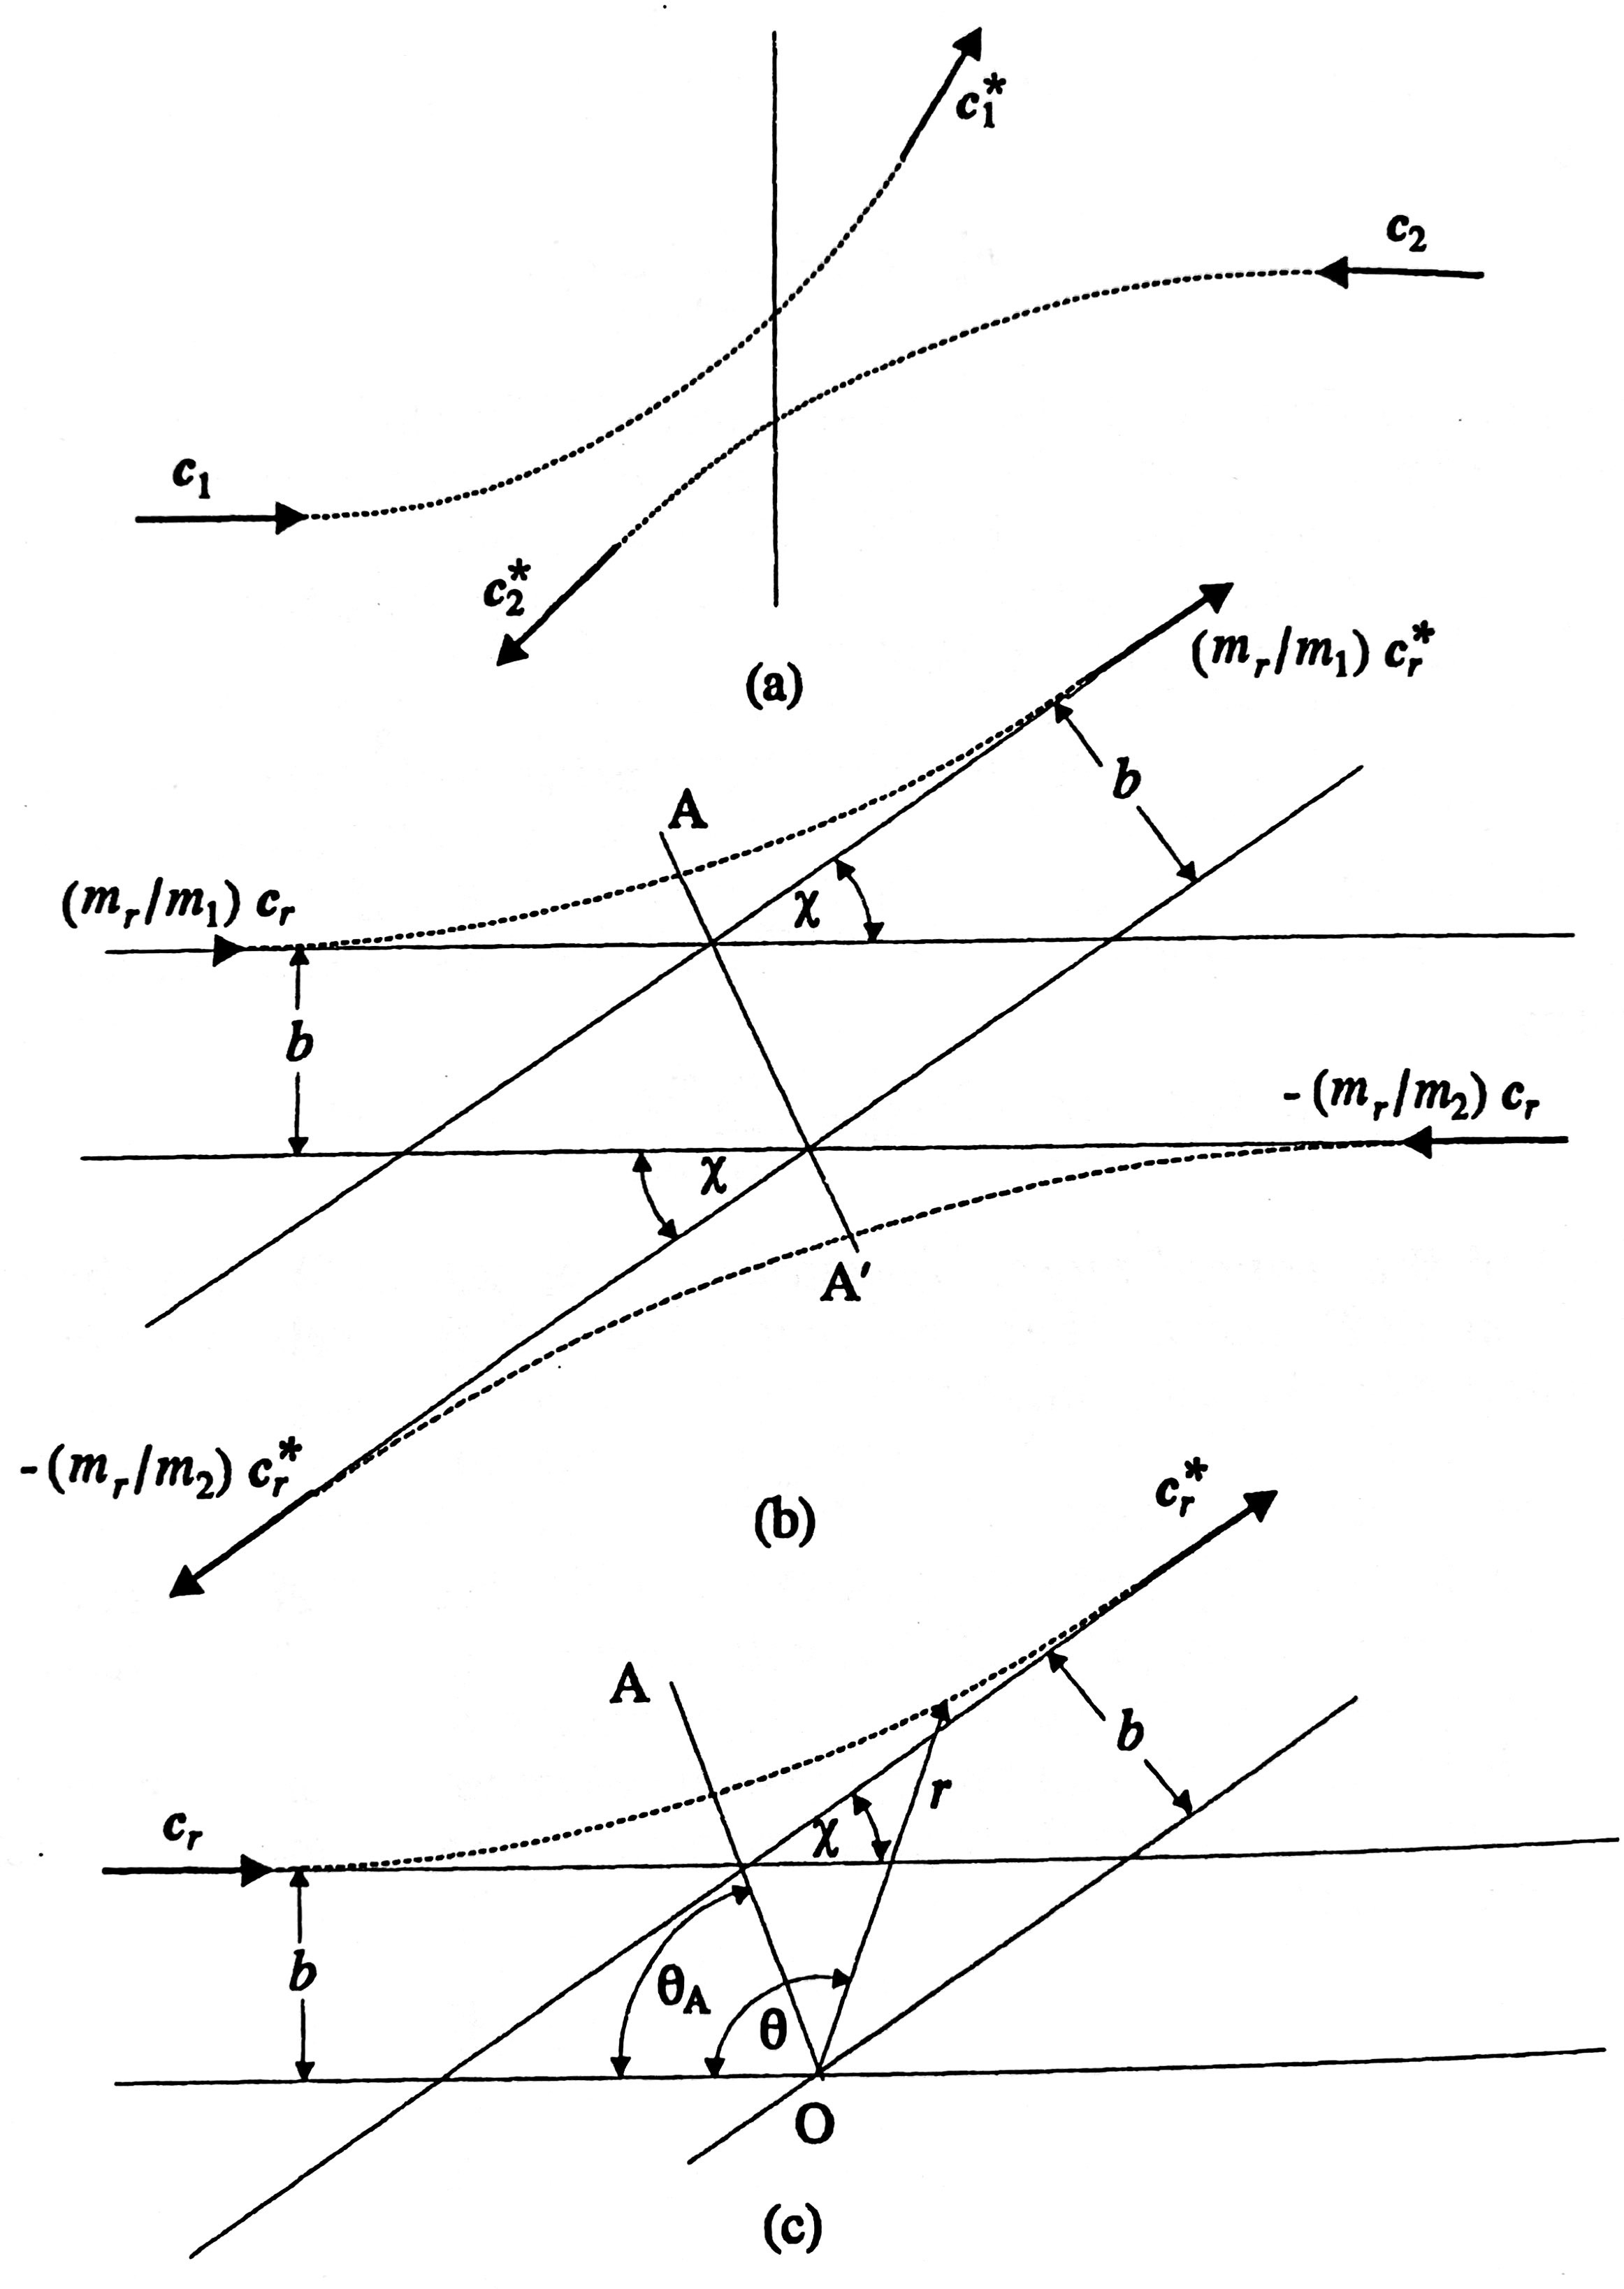
\includegraphics[width=10cm]{fig/dsmc/bird1.jpg}
    \caption{2体衝突の表現 : (a) 基準となる実験系,(b) 基準の重心座標系での2体衝突,(c) 換算質量粒子と固定散乱中心の相互作用~\cite{bird1994molecular}.}
    \label{fig:bird1}
\end{figure}

\subsection{衝撃パラメータと衝突断面積}
2つの分子の速度を分離して,弾性衝突を表すためには2つの衝撃パラメータが必要となる.
1つ目は,重心座標系での乱れていない軌道の最も近いアプローチ$b$の距離で,
2つ目は,Collision planeとReference planeの角度$\varepsilon$である.
ただし,分子の衝突前および衝突後の軌道は,同じ平面である.

パラメータ$b$および$\varepsilon$は,特定の偏向角$\chi$を与える.
パラメータ$b$と$\varepsilon$に対応する微分断面積$\sigma \mathrm{d}\Omega$は,
\begin{equation}
    \sigma \mathrm{d}\Omega = b{\rm d}b\mathrm{d}\varepsilon,
\end{equation}
であり,$\mathrm{d}\Omega$はベクトル$c_r^*$方向の微小立体角である.
図~\ref{fig:bird2}より,
\begin{equation}
    \mathrm{d}\Omega = \sin \chi\mathrm{d}\chi\mathrm{d}\varepsilon,
\end{equation}
従って,
\begin{equation}
    \sigma = \dfrac{b}{|\sin\chi|}\dfrac{\mathrm{d}b}{\mathrm{d}\chi}.
\end{equation}
また,全衝突断面積$\sigma_T$は次式で表される.
\begin{equation}
    \sigma_T = \int_0^{4\pi}\sigma\mathrm{d}\Omega = 2\pi\int_0^\pi \sigma\sin\chi\mathrm{d}\chi.
\end{equation}
さらに粘性係数の断面積$\sigma_\mu$は次式のようになる.
\begin{equation}
    \sigma_\mu = \int_0^{4\pi}\left( \sin^2 \chi \right)\sigma\mathrm{d}\Omega 
    = 2\pi\int_0^\pi \left(\sin^3 \chi\right)\sigma\sin \chi\mathrm{d}\chi.
\end{equation}
衝突前の速度方向に垂直となる衝突後の速度成分は$c_r\sin \chi$である.
この積分は,粘性係数を算出するために,Chapman–Enskog理論~\cite{bird1994molecular}で用いられる.

拡散断面積とも呼ばれる運動量輸送断面積は,
\begin{equation}
    \sigma_M = \int_0^{4\pi}\left(1 - \cos \chi\right)\sigma\mathrm{d}\Omega 
    = 2\pi\int_0^\pi \left(1-\cos \chi\right)\sin \chi\mathrm{d}\chi.
\end{equation}
粘性係数の断面積と同様にして,
衝突前の速度方向に垂直となる衝突後の速度成分は$c_r\left(1 - \cos \chi\right)$である.
この積分は,拡散係数を算出するために,Chapman–Enskog理論~\cite{bird1994molecular}で用いられる.

\begin{figure}
    \centering
    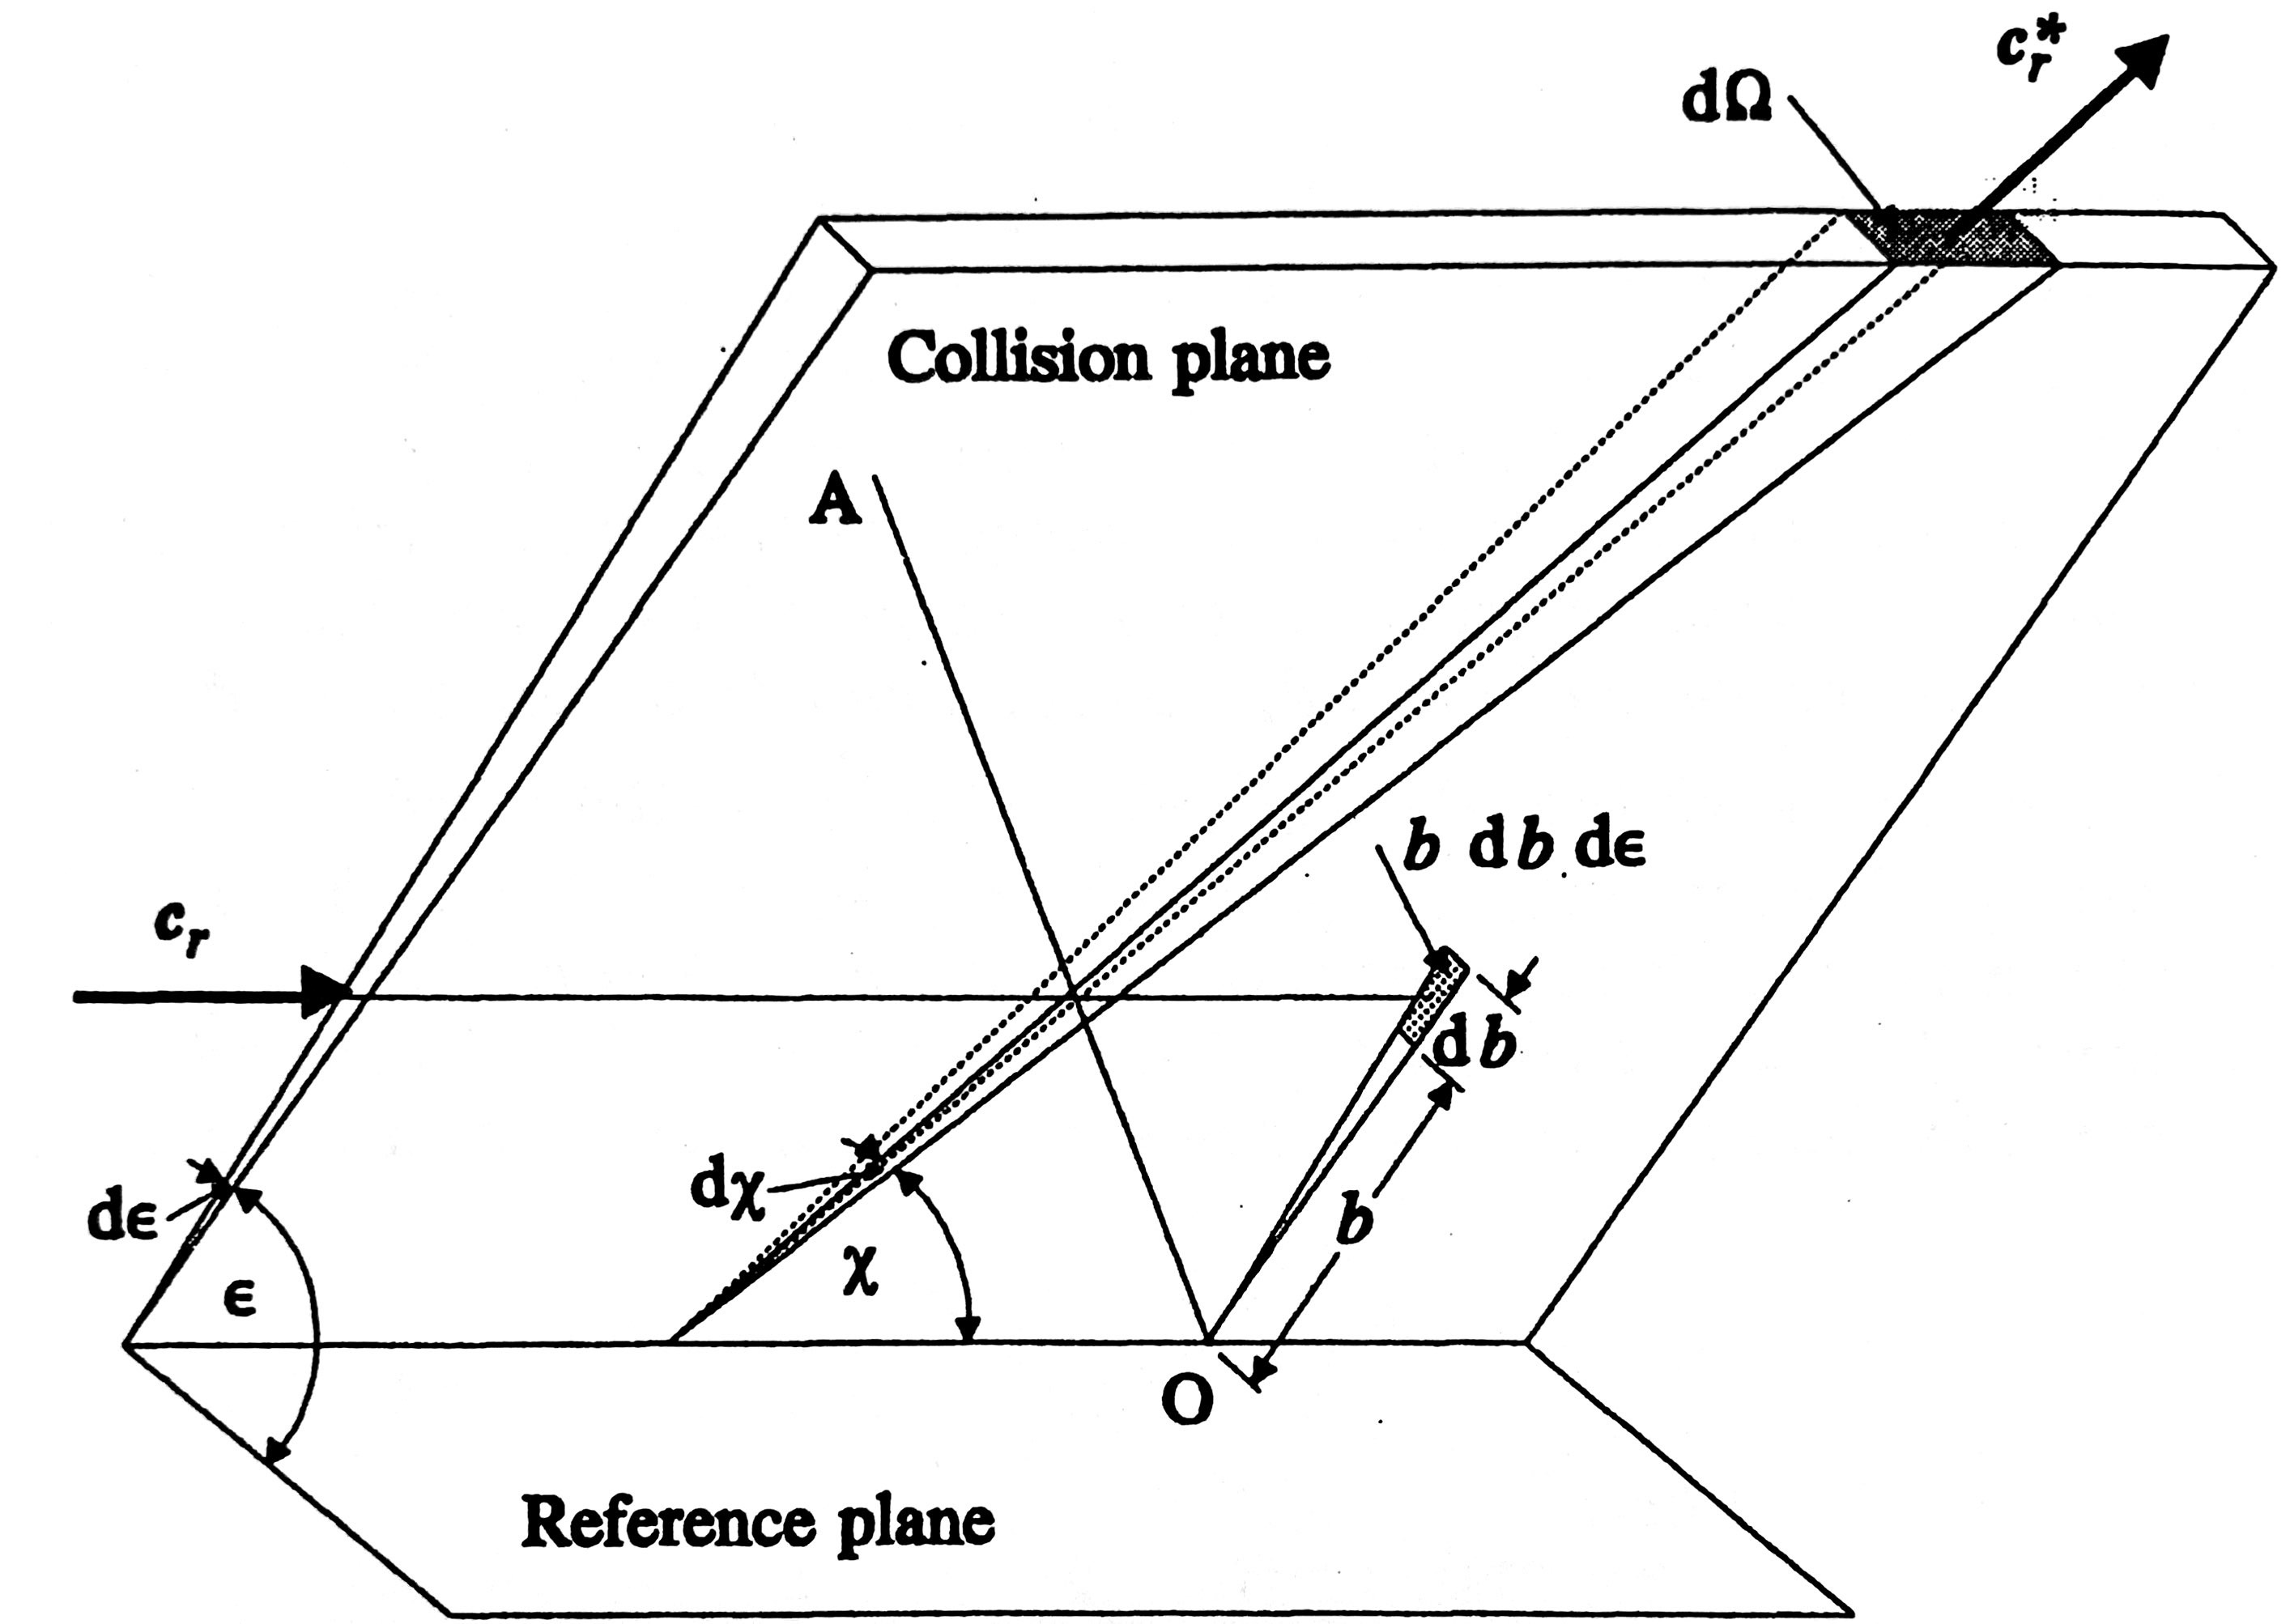
\includegraphics[width=10cm]{fig/dsmc/bird2.jpg}
    \caption{衝突パラメータ~\cite{bird1994molecular}.}
    \label{fig:bird2}
\end{figure}

\subsection{Variable Soft Sphere モデル}
DSMC法における衝突は,物理モデルと計算効率の双方を考慮した分子モデルを選択する必要がある.
近年のDSMC法で一般に用いられる分子モデルとして,
KouraとMatsumoto~\cite{koura1991variable}により提唱されたVariable Soft Sphere (VSS) モデルがある.
VSSモデルでは接触の瞬間に無限の反発力を持ち,
それ以外の場合は力を及ぼさない弾性球として分子を扱う.
このモデルでは分子の直径$d$と相対速度$c_r$の関係は以下のようになる.
\begin{equation}
    d \propto c_r^{(1/2)-\omega}.
\end{equation}
ただし,$\omega$はモデルパラメータである.
また,偏向角は衝突パラメータ$b$を用いて次式のようになる.
\begin{equation}
    \chi = 2\cos^{-1}\left(\dfrac{b}{a}\right)^{1/a}.
\end{equation}
ここで,$a$はVSSモデルの散乱パラメータで,VSSモデルでの全衝突断面積は
$\sigma_T  = \pi d^2$で与えられる.
これによりVSSモデルでの粘性係数が求められて,
\begin{equation}
    \mu=\dfrac{5}{16} \frac{(\alpha+1)(\alpha+2) \sqrt{\pi m k}\left(\frac{4 k}{m}\right)^{\xi} T^{\frac{1}{2}+\xi}}{\alpha \Gamma(4-\xi) \sigma_{T, \mathrm{ref}} c_{r, \mathrm{ref}}^{2 \xi}},
\end{equation}
となる.

VSSモデルは単純でかつ,
平衡~\cite{gallis2004molecular}および非平衡~\cite{gallis2011investigation}両方の条件下で単原子分子の輸送特性を正確に予測できるため,DSMC法で良く用いられる.
さらに,より現実的であるが計算コストがより高いLennard–JonesポテンシャルやMorseポテンシャルと比較すると計算効率がより高いという特徴もあり,
本研究ではVSSモデルを使用する.

\begin{table}[H]
    \centering
    \caption{本研究で用いるVSSモデルのパラメータ}
    \begin{tabular}{c|cccc}
    \hline\hline
        化学種 & $d$~[m] & $\omega$~[$-$] & $T_\mathrm{ref}$~[K] & $\alpha$~[$-$] \\ \hline
        \ce{O2} & \num{3.96d-10} & 0.77 & 273.15 & 1.4 \\
        \ce{N2} & \num{4.07d-10} & 0.77 & 273.15 & 1.6 \\
        \ce{O} & \num{3.00d-10} & 0.77 & 273.15 & 1.0 \\
        \ce{N} & \num{3.00d-10} & 0.77 & 273.15 & 1.0 \\
        \ce{NO} & \num{4.00d-10} & 0.77 & 273.15 & 1.0 \\
        \hline\hline
    \end{tabular}
    \label{tab:vss}
\end{table}

\subsection{内部エネルギー}
多原子分子においては内部エネルギーモードが存在するため,
多原子分子の衝突を記述するには並進および内部のエネルギー状態との緩和断面積が必要である.
ただし,全ての断面が分かっている場合でも,多数の遷移があるためこの方法は複雑化する.

多原子分子を効率よく計算する方法としては,単原子分子のモデルに多原子分子の機能を追加するという手法がある.
従って,VSSモデルに内部エネルギーモードと並進および内部エネルギー交換を行う方法を追加することで,多原子分子へと拡張する.
内部エネルギーモードは自由度$\xi$によって特徴付けられる.

DSMC法においては,現象論的なLarsen–Borgnakke(GLB)モデルがエネルギー交換に用いられる.
このGLBモデルでの非弾性衝突後の内部エネルギーは,
全エネルギーの平衡分布からサンプリングし以下のように割り当てられる.
\begin{align}
f\left(\dfrac{E_{t r}}{E_{c}}\right) &= \dfrac{\Gamma[5 / 2-\omega+\zeta]}{\Gamma[5 / 2-\omega] \Gamma[\zeta]}\left(\dfrac{E_{t r}}{E_{c}}\right)^{3 / 2-\omega}\left(1-\dfrac{E_{t r}}{E_{c}}\right)^{\zeta-1} \\
f\left(\dfrac{E_{i}}{E_{c}}\right) &= \dfrac{\Gamma[5 / 2-\omega+\zeta]}{\Gamma[5 / 2-\omega] \Gamma[\zeta]}\left(1-\dfrac{E_{i}}{E_{c}}\right)^{3 / 2-\omega}\left(\dfrac{E_{i}}{E_{c}}\right)^{\zeta-1}
\end{align}
ただし,$E_{tr}$は並進エネルギー,$E_i$は内部エネルギー,$E_c = E_{tr} + E_i$は衝突分子ペアの
全エネルギー,$\gamma$はガンマ関数である.
衝突モデルは,$\omega$を介して平衡分布となるため,
平衡分布を実際に衝突している分子の分布から区別している~\cite{bird1994molecular}.

回転エネルギーと異なり,
並進エネルギーよりも広い間隔のエネルギー状態を持つため,振動モードは完全には励起されない.
従って,エネルギー状態を連続的に記述するよりも離散的な記述が必要である.
2原子分子の振動モードの離散的なエネルギー状態は,それぞれがポテンシャルおよび運動エネルギーから影響され,
調和振動子モデルおよび非調和振動子モデルを使用して記述される.

\subsection{化学反応モデル}
空気の中性粒子そのイオンから成るNASA Air–11混合気体の化学反応は,
Parkのメカニズムによって説明されている~\cite{park1993review,park2001chemical}.
このメカニズムには一酸化窒素の解離反応が考慮されており,
流星周りにおける一酸化窒素の存在は過去に研究がなされている~\cite{menees1976nitric,park1978odd,silber2018nitric}.

本研究における化学反応はBird~\cite{bird1994molecular}によるTotal Collision Energy (TCE) 法を用いる.
TCEモデルでは既知の反応係数に基づいて反応確率を定義する.

%\subsection{速度分布関数}
%期待中の分子すべてが同じ速度で運動しているわけではないため,分子運動を取り扱い祭にはどの速度をもった分子がどれくらい存在するかを表す速度分布関数が必要になる.
%位置を$\bm{x}$とすると,ある位置での分子数密度は$n(\bm{x})$と書ける.
%その位置を含む微小検査体積$\mathrm{d}v = \mathrm{d}x\mathrm{d}y\mathrm{d}z$の中にある分子の数は$n(\bm{x})\mathrm{d}v$になる.
%分子の速度$c$の直交座標成分を$c_1,\ c_2,\ c_3$として,それぞれを座標軸とした速度空間を考え,
%ある速度空間でのベクトル$\bm{c}$の先端に体積$\mathrm{d}c = \mathrm{d}c_1\mathrm{d}c_2\mathrm{d}c_3$の直方体を考える.
%この中にある分子の数は分子速度関数$f$を用いて$fn\mathrm{d}c$と書くことができ,$c\sim c+\mathrm{d}c$の速度を持つ分子の数を表す.$f$は速度空間の市によって変わるため$c$の関数であり,
%速度空間すべての分子数を加えると全体の分子数に等しいという以下に示す条件を満たす必要がある.
%\begin{equation}
%    \int^\infty_{-\infty}\!\int^\infty_{-\infty}\!\int^\infty_{-\infty}
%    fn\mathrm{d}c = n
%\end{equation}
%
%非定常流れでは$n$は時間$t$の関数でもあるため,それに伴って$f$も位置と時間の関数になる.

\subsection{SPARTAカーネル}
DSMC法を実行可能なオープンソースコードとして,
MONACO~\cite{padilla2010comparison}やDAC~\cite{padilla2010comparison},dsmcFoam(+)~\cite{scanlon2010open,white2018dsmcfoam+,raeisi2019numerical}などがあるが,
本研究におけるDSMC法の計算コードにはSPARTAカーネル~\cite{spartaWWW,bariselli2020aerothermodynamic,plimpton2019direct}を用いた.
SPARTAはGPLライセンスのオープンソースソフトウェアとして配布され,
単列計算または,MPIライブラリを用いた領域分割による並列計算が可能である.
DSMC法への理解と入力ファイルの記述が必要になる.

入力ファイルは以下のような4つの手順によって記述される.
\begin{enumerate}
    \item 初期化
    \item 問題定義
    \item 条件設定
    \item シミュレーションの開始
\end{enumerate}
3番目および4番目の手順は計算が収束するまで反復することができる.

\subsubsection{1. 初期化}
ここでは,シミュレーションに必要なパラメータの設定を行う.
ここで設定するパラメータは単位系 (CGS単位系またはSI単位系),
乱数に用いるシード値,
計算領域の次元 (2次元または3次元) が含まれる.

\subsubsection{2. 問題定義}
ここでは,シミュレーションの開始に必要となる全てのパラメータを設定する.
計算領域となるボックスの大きさ,
計算領域境界におけるサンプル粒子の振る舞い,
格子数の設定,
計算領域内部における固体表面の設置,
粒子の分子組成と初期状態の設定などが含まれる.

\subsubsection{3. 条件設定}
初期化および問題定義の次は入力ファイルでの条件設定を行う.
ここでは,出力方法や出力する物理量,
衝突モデル,化学モデル,並列計算での動的負荷分散,
境界条件,固体表面での反射モデルの選択などを定義する.
この部分はシミュレーション結果の品質に大きく関わり,重要である.
さらにこの部分では,
固体表面の特性計算,時間刻み幅,サンプリング間隔も具体的に定義する.
サンプリング間隔の設定が適切に行われないと結果の品質が著しく低下し,
出力結果の書き込み頻度は計算時間に大きく影響するため慎重に指定する必要がある.

